\documentclass[
  overfullrule,
  12pt,
  a4paper,
  twoside,
  BCOR=8mm,
  numbers=noenddot,
  chapterprefix=true,
  headings=small,
  headsepline,
  bibliography=totoc,
  listof=totoc,
  markcase=upper, % make listof headings uppercase
]{scrbook}

\usepackage{scrlayer-scrpage}
\usepackage{scrtime} % \thistime on title page

\usepackage[utf8]{inputenc} % Use UTF-8 as input file encoding
\usepackage[T1]{fontenc} % Use Type 1 (8bit) fonts
\usepackage[ngerman,american]{babel} % Language settings
\usepackage[final]{microtype} % Fix many overfull hboxes

\usepackage[defaultsans,scale=0.9]{lato} % Use Lato as sans-serif font
\usepackage{fourier} % Use Adobe Utopia as standard font
\usepackage[scaled=0.83]{beramono} % Use Bera Mono as monospace font

\usepackage[
  style=numeric-comp,
  backref=true,
]{biblatex}
\addbibresource{stuff.bib}
\usepackage{csquotes}

%\usepackage{todonotes}

\usepackage{etoolbox} % \ifblank
\usepackage{xparse} % \NewDocumentCommand
\usepackage{mathtools} % Math improvements, loads amsmath
\usepackage{amssymb} % \mathbb
\usepackage{amsthm}
\usepackage{thmtools} % \listoftheorems
\usepackage{array} % >{...} column modifiers
\usepackage{siunitx}
\usepackage{booktabs} % \toprule etc
\usepackage{xspace}
\usepackage{enumitem} % improved listings: \setlist
\usepackage{listings,xcolor} % source code
\usepackage{subcaption} % subfigure
\usepackage[nottoc]{tocbibind} % remove toc from toc (caused by algorithm2e)
\usepackage[
  linesnumbered,
  algochapter,
  dotocloa,
  norelsize, % line numbers in \scriptsize
]{algorithm2e}

% hyperref should be loaded last
\usepackage[
  bookmarksopen,
  bookmarksopenlevel=0, % close all
  bookmarksnumbered,
]{hyperref}

% glossaries must be loaded after hyperref
\usepackage[toc,shortcuts]{glossaries}

\mathtoolsset{
  %showonlyrefs,
  showmanualtags,
}

\sisetup{
  binary-units,
  round-mode = places,
  round-precision = 2,
}

\hypersetup{
  %hidelinks, %TODO: activate me for print version
}

\usetikzlibrary{graphs,arrows.meta}
\tikzset{>=Stealth}

% hyperref/babel/koma
\renewcaptionname{american}\chapterautorefname{Chapter}
\renewcaptionname{american}\sectionautorefname{Section}
\renewcaptionname{american}\subsectionautorefname{Subsection}
\newcaptionname{american}\algorithmcflinename{step} % algorithm2e

\newcommand{\N}{\mathbb{N}} % Natural numbers
\newcommand{\Z}{\mathbb{Z}} % Whole numbers
\newcommand{\Q}{\mathbb{Q}} % Rational numbers
\newcommand{\R}{\mathbb{R}} % Real numbers
\newcommand{\C}{\mathbb{C}} % Complex numbers
\newcommand{\F}{\mathbb{F}} % Arbitrary Field
\newcommand{\K}{\mathbb{K}} % Arbitrary Field

\newcommand{\Cneg}{\C_-} % Negative Half Plane

\newcommand{\im}{i} % imaginary unit

\newcommand{\onehalf}{\tfrac{1}{2}}

% matrices
\newcommand\Cnn{\C^{n\times n}}
\newcommand\Rnn{\R^{n\times n}}
\newcommand\Rnr{\R^{n\times r}}
\newcommand\Rnk{\R^{n\times k}}
\newcommand\Rkk{\R^{k\times k}}
\newcommand\nnz{\operatorname{nnz}}
\renewcommand\vec{\operatorname{vec}}
\DeclareMathOperator{\colspan}{span}
\DeclareMathOperator{\orth}{orth}
\DeclareMathOperator{\rank}{rank}
\DeclareMathOperator{\diag}{diag}
\newcommand\MP{\dagger} % Moore Penrose pseudo-inverse

% transpose and conjugate/Hermitian transpose:
\newcommand\conj[1]{\overline{\optional{#1}}}
\newcommand\T{T}
\newcommand\HT{H}

% Rosenbrock
\newcommand\Ham{\ensuremath{H}}
\newcommand\Ricc{\operatorname{\mathcal R}}
\newcommand\Jac{\operatorname{\mathcal J}}

 % ADI
\newcommand\Aip{\mathop{H_k^+}}
\newcommand\Aim{\mathop{H_k^-}}
\newcommand\Aipm{\mathop{H_k^\pm}}
\newcommand\Aiip{\mathop{V_k^+}}
\newcommand\Aiim{\mathop{V_k^-}}
\newcommand\Aiipm{\mathop{V_k^\pm}}
\newcommand\Cayley{\mathop{\mathcal{C}}}
\newcommand\Aipinv{\mathop{(\Aip)^{-1}}}
\newcommand\Aiipinv{\mathop{(\Aiip)^{-1}}}
\newcommand\Lyap{\operatorname{\mathcal L}}

% usage: \{2x\given x\in\N}
\newcommand{\given}{\mid}

% usage: \Set[\big]{2x \given x\in\N}
\newcommand\SetSymbol[1][]{%
  \nonscript\:#1\vert
  \allowbreak
  \nonscript\:
  \mathopen{}}
\DeclarePairedDelimiterX{\Set}[1]{\lbrace}{\rbrace}{%
  \renewcommand\given{\SetSymbol[\delimsize]}% this effect is local only
  #1%
}

% personal taste:
\let\epsilon\varepsilon
%\renewcommand{\to}{\longrightarrow}
%\renewcommand{\mapsto}{\longmapsto}
%\renewcommand{\gets}{\longleftarrow}
\renewcommand{\Re}{\operatorname{Re}} % real part of a complex number
\renewcommand{\Im}{\operatorname{Im}} % imaginary part

% some more delimiters:
\NewDocumentCommand{\optional}{m}{\ifblank{#1}{\,\cdot\,}{#1}}
\DeclarePairedDelimiterX{\abs}[1]{\lvert}{\rvert}{\optional{#1}}
\DeclarePairedDelimiterX{\norm}[1]{\lVert}{\rVert}{\optional{#1}}
\DeclarePairedDelimiterX{\scalar}[2]{\langle}{\rangle}{\optional{#1},\optional{#2}}
\newcommand{\card}{\abs}

% integration:
\NewDocumentCommand{\intd}{m}{\,\textup{d}#1}
\newcommand\dt{\intd{t}}

% differentiation:
\NewDocumentCommand{\pdiff}{mm}{\frac{\partial #2}{\partial #1}}
\NewDocumentCommand{\diff}{mm}{\frac{\mathrm{d} #2}{\mathrm{d} #1}}

% https://tex.stackexchange.com/questions/22561/what-is-the-proper-use-of-i-e-backslash-at?noredirect=1&lq=1
\makeatletter % no idea why this is needed. \@ifnextchar doesn't work without it.
\newcommand\cf{cf.\@\xspace} % confer
\newcommand\eg{e.g.\@\xspace} % exempli gratia
\newcommand\etc{etc\@ifnextchar.{}{.\@\xspace}} % et cetera
\newcommand\ie{i.e.\@\xspace} % id est
\newcommand\wrt{w.r.t.\@\xspace} % with respect to
\makeatother

\hyphenation{pa-ra-me-tri-zed}
\hyphenation{pa-ra-bo-lic}
\hyphenation{para-real}
\hyphenation{pipe-line}
\hyphenation{Syl-ves-ter}
\hyphenation{in-qui-ries}

% Remember: use \label{thm:...} for theorems, propositions, lemmata, etc.
% This way the type of an environment can easily be changed.

\declaretheoremstyle[
  spaceabove = \topsep,
  spacebelow = \topsep,
  postheadspace = 0.5em, % matches proof
  headfont = \usekomafont{captionlabel},
  notefont = \normalfont\sffamily,
  bodyfont = \normalfont,
  qed = \ensuremath{\triangle\hspace*{-.1ex}}, % bring it a little bit closer to the edge
]{myplain}

\declaretheoremstyle[
  spaceabove = \topsep,
  spacebelow = \topsep,
  postheadspace = 0.5em, % matches proof
  headfont = \itshape,
  numbered = no,
  qed = \ensuremath{\triangle\hspace*{-.1ex}}, % bring it a little bit closer to the edge
]{myremark}

\renewcommand{\qedsymbol}{\ensuremath{\square}} %TODO: still not bold enough compared to \triangle

\declaretheorem[style=myplain, numberwithin=chapter]{lemma}
\declaretheorem[style=myplain, numberlike=lemma]{corollary}
\declaretheorem[style=myplain, numberlike=lemma]{proposition}
\declaretheorem[style=myplain, numberlike=lemma]{theorem}
\declaretheorem[style=myplain, numberlike=lemma]{hypothesis}

\declaretheorem[style=myplain, numberlike=lemma]{definition}
\declaretheorem[style=myplain, numberlike=lemma]{example}

\declaretheorem[style=myremark]{remark}


% ******************************************************************************
% Listings

\setlist[enumerate]{font=\normalfont}
\setlist[enumerate,1]{label=(\roman*)}
\setlist[enumerate,2]{label=(\alph*)}
\setlist[enumerate,3]{label=(\arabic*)}


% ******************************************************************************
% Source Code

\renewcommand{\lstlistlistingname}{List of Code Snippets}
\renewcommand{\lstlistingname}{Code Snippet}

\lstset{
  basicstyle=\small\ttfamily,
  numberstyle=\scriptsize\sffamily, % matches algorithm2e
  numbers=left,
  % use special julia comments as range markers: #== text ==#
  rangeprefix=\#\=\=\ ,
  rangesuffix=\ \=\=\#,
  includerangemarker=false,
  % add latex labels using #* \label{line:...}
  escapeinside={\#*}{\^^M},
}

% ******************************************************************************
% algorithm2e

\setlength{\algomargin}{0pt}

\newcommand{\komacaptionsty}{\usekomafont{captionlabel}}
\SetAlCapFnt{\usekomafont{captionlabel}}
\SetNlSty{textsf}{}{} % matches listings
\SetKwSty{komacaptionsty}
\SetCommentSty{normalfont}
\SetArgSty{normalfont} % used for conditions as well

\makeatletter
% Fix alignment of listofalgorithms:
\renewcommand*\l@algocf{\@dottedtocline{1}{1.5em}{2.3em}}
% Thanks to https://tex.stackexchange.com/a/147750/95100
\renewcommand{\@algocf@capt@plain}{above}% formerly {bottom}
\makeatother

\AtBeginDocument{
  \DontPrintSemicolon
  \SetAlgorithmName{Algorithm}{Algorithm}{List of Algorithms}
  \SetKwComment{Comment}{}{}
}

\newcommand\julia\texttt
\newcommand\code\texttt

\newcommand\LDLt{LDL\textsuperscript{T}}

\counterwithout*{footnote}{chapter}
\setcounter{topnumber}{1} % max number of floats at top of page
\renewcommand{\bottomfraction}{0.5}
\renewcommand{\listtheoremname}{List of Theorems and Examples}

\newcommand\LandauO{\operatorname{\mathcal O}}

% runtime estimates
\newcommand\hattpar{\hat t_\text{par}} % estimate
\newcommand\hattseq{\hat t_\text{seq}} % estimate
\newcommand\tpar{t_\text{par}}
\newcommand\tseq{t_\text{seq}}
\newcommand\twarmup{t_\text{warm-up}}
\newcommand\trampup{t_\text{ramp-up}}
\newcommand\JIT{\operatorname{compile}}

% error estimates
\newcommand\umach{\mathrm u_\text{mach}} % machine precision

\renewcommand{\bfdefault}{eb}

% Use Lato Extra Bold
\setkomafont{disposition}{\sffamily\bfseries}

% Header and footer font
\setkomafont{pageheadfoot}{\footnotesize\sffamily\bfseries}
\setkomafont{pagenumber}{\footnotesize\sffamily\bfseries}

% Captions of tables, figures etc.
\setkomafont{captionlabel}{\sffamily\bfseries}
\setkomafont{chapterprefix}{\normalfont\normalsize\sffamily\MakeUppercase}

% Header and footer content
\automark[chapter]{chapter}
\renewcommand{\chaptermark}[1]{%
  \markboth{\bfseries\MakeUppercase{\chapappifchapterprefix{~}}\thechapter\mdseries\quad\MakeUppercase{#1}}%
           {\mdseries\MakeUppercase{#1}\quad\bfseries\MakeUppercase{\chapappifchapterprefix{~}}\thechapter}}


\makeglossaries

% props to:
% https://tex.stackexchange.com/questions/567985/problems-with-inputtable-tex-hline-after-2020-fall-latex-release
% https://tex.stackexchange.com/questions/144625/misplaced-noalign-error-in-table-but-only-when-using-include
\makeatletter\let\expandableinput\@@input\makeatother

\begin{document}

% -----------------------------------------------------------------------------
\frontmatter

\begin{titlepage}
  %FIXME: Fix the two-sided layout for the title page;
  % this is local to the titlepage environment
  \oddsidemargin  8mm
  \evensidemargin 0mm

  \begin{center}
    \renewcommand{\baselinestretch}{1.2}%
    \LARGE%

    {\Large\sffamily Master Thesis}\\
    {\huge\sffamily\bfseries A Low-Rank Parareal Solver for} \\
    {\huge\sffamily\bfseries Differential Riccati Equations} \\
    {\huge\sffamily\bfseries Written in Julia}
    \vskip 12mm%

    {\Large\sffamily in partial fulfillment of the requirements} \\
    {\Large\sffamily for the degree Master of Science} \\
    {\Large\sffamily at the Faculty of Mathematics of the } \\
    {\LARGE\sffamily\bfseries Otto-von-Guericke-Universität Magdeburg}

    \vfill%

    {\large submitted by}\\
    {\Large Jonas Schulze}\\
    \bigskip
    {\large \begin{tabular}{rl}
      Date of Birth & August 22, 1995 \\
      Course of Studies & \foreignlanguage{ngerman}{Mathematik} \\
      Branch of Studies & \foreignlanguage{ngerman}{Computermathematik} \\
      Date of Submission & April 12, 2022 \\[3\bigskipamount] %TODO: change me before printing
      Supervisor & Dr.~Martin Köhler\\
      Reviewer & Prof.~Dr.~Peter Benner\\
    \end{tabular}}\\
  \end{center}
\end{titlepage}


\thispagestyle{empty}
\vspace*{\fill}
\section*{Statement of Authorship}

\begin{foreignlanguage}{ngerman}
Hiermit erkläre ich, dass ich die vorliegende Arbeit selbstständig und ohne
Benutzung anderer als der angegebenen Quellen und Hilfsmittel angefertigt habe.

Die vorliegende Arbeit ist frei von Plagiaten.
Alle Ausführungen, die wörtlich oder inhaltlich aus anderen Schriften entnommen sind,
habe ich als solche kenntlich gemacht.

Diese Arbeit wurde in gleicher oder ähnlicher Form noch bei keinem anderen
Prüfer als Prüfungsleistung eingereicht und ist auch noch nicht veröffentlicht.

\vspace*{3cm}
\noindent
\parbox{5cm}{\centering\footnotesize\dotfill\\Jonas Schulze}
\end{foreignlanguage}

%\chapter{Abstract}

Get a parareal solver running with column compression.
The tricky part is that the interface solutions (solutions at time slice bounds) differ in size,
\wrt both storage requirements and matrix dimensions.


\cleardoublepage
\pdfbookmark{\contentsname}{toc} % add toc to bookmarks, but not to toc
\tableofcontents
\listofalgorithms
\lstlistoflistings
\listoffigures
\listoftables

\cleardoublepage
\pdfbookmark{\listtheoremname}{loe}
\listoftheorems[ignore=remark]

\chapter*{Glossary}
\addcontentsline{toc}{chapter}{Glossary}
\printglossary[title=Abbreviations]

\markboth{\bfseries GLOSSARY}{\bfseries GLOSSARY}

\section*{Numbers and Vector Spaces}

\noindent
\begin{tabular}{@{}p{2.5cm}l}
  $\N$ & set of natural numbers. \\
  $\R$ & field of real numbers. \\
  $\C$ & field of complex numbers. \\
  $\Cneg$ & left complex half plane, $\Cneg := \Set{z\in\C : \Re(z) < 0}$. \\
  $\K^n$ & vector space of $n$-tuples having entries in $\K$. \\
  $\K^{m\times n}$ & vector space of $m\times n$ matrices having entries in $\K$. \\
  $\im$ & imaginary unit, $\im^2 = -1$. \\
  $\conj{(\optional{})}$ & complex conjugate of a scalar or matrix, $\conj{a + b\im} := a - b\im$ for $a,b\in\R$. \\
  $\Re(\optional{}) / \Im(\optional{})$ & real/imaginary part of a scalar or matrix, \\
    & $\Re(a + b \im) := a$, $\Im(a+b\im) := b$ for $a, b\in\R$.
\end{tabular}

\section*{Norms}

\noindent
\begin{tabular}{@{}p{2.5cm}l}
  $\abs{}$ & absolute value of a scalar. \\
  $\norm{}_2$ & Euclidean norm of a vector, $\norm{x}_2 := \sqrt{x^\HT x}$ for $x\in\R^n$, or \\
              & spectral norm of a matrix, $\norm{A}_2 := \max_{\norm{x}_2 = 1} \norm{Ax}_2 = \rho(A)$. \\
  $\norm{}_F$ & Frobenius norm of a vector or matrix, $\norm{X}^2_F := \sum_{i,j} \abs{x_{ij}}^2$.
\end{tabular}

\section*{Matrices}

\noindent
\begin{tabular}{@{}p{2.5cm}l}
  $I_n$ & identity matrix of size $n\in\N$. \\
  $\mathrlap{(\optional{})^\T} \hphantom{(\optional{})^{-\T}} / (\optional{})^\HT$ & transpose / Hermitian transpose of a matrix. \\
  $(\optional{})^{-\T} / (\optional{})^{-\HT}$ & inverse of the transpose / Hermitian transpose of a (square) matrix. \\
  $(\optional{})^{-1}$ & inverse of a (square) matrix. \\
  $(\optional{})^\MP$ & Moore-Penrose pseudo inverse of a matrix. \\
  $\rank(\optional{})$ & rank of a matrix. \\
  $\colspan(\optional{})$ & vector space spanned by the columns of a matrix. \\
  $\Lambda(\optional{}) / \Lambda(\optional{},\optional{})$ & spectrum of a matrix / matrix pair,\\
    & $\Lambda(A) := \Lambda(A, I)$, $\Lambda(A, E) := \Set{\lambda\in\C \given \exists v : Av = \lambda Ev}$. \\
  $\rho(\optional{})$ & spectral radius of a matrix, $\rho(G) := \max\Set[\big]{\abs{\lambda} : \lambda\in\Lambda(G)}$. \\
  $\nnz(\optional{})$ & number of non-zero entries of a matrix.
\end{tabular}

\section*{Relations}

\noindent
\begin{tabular}{@{}p{2.5cm}l}
  $X \succeq 0 / Y \succ 0$ & positive semi-definite matrix $X$ / positive definite matrix $Y$, \\
    & $\Lambda(X) \subseteq \Set{\lambda\in\R : \lambda\geq 0}$, $\Lambda(Y) \subseteq \Set{\lambda\in\R : \lambda > 0}$. \\
  $f(x) \mathrel{\smash{\overset{!}{\Delta}}} 0$ & determine $x$ such that $f(x) \mathrel{\Delta} 0$ holds, where $\Delta\in\Set{=,\succ}$ is a relation. \\
  $\ll$ & much less than. \\
  $\equiv$ & pointwise equality of functions. \\
  $\cong$ & equality up to an isomorphism.
\end{tabular}

\section*{Derivatives}

\noindent
\begin{tabular}{@{}p{2.5cm}l}
  $\vphantom{\smash[t]{\Big(}} f'(x) := \diff{x}{f}(x)$ & first derivative of $f$. \\
  $\vphantom{\smash[t]{\Big(}} \dot x := \diff{t}{x}$ & derivative of $x$ \wrt time $t$. \\
  $\vphantom{\smash[t]{\Big(}} V_z := \pdiff{z}{V}$ & partial derivative of $V$ \wrt $z$. \\
  $V_z(t,z) |_{z=x} $ & partial derivative of $V$ \wrt $z$, evaluated at $(t,z)=(t,x)$.
\end{tabular}

\section*{Variables and Constants}

\noindent
\begin{tabular}{@{}p{2.5cm}l}
  $k$ & ADI or parareal step. \\
  $k_n$ & last parareal refinement $U^{k_n}_n$ computed by stage $n$. \\
  $K$ & depending on the context: \\
    & feedback matrix $K(t) := R^{-1} B^T X(t) E \in\R^{m\times n}$, or \\
    & maximum number of parareal steps/refinements allowed, $k\leq K$. \\
  $m$ & number of system controls $u(t)\in\R^m$, $m\ll n$. \\
  $n$ & depending on the context: \\
    & number of system states $x(t)\in\R^n$, or \\
    & specific time step $t_n$, $1 \leq n \leq N$. \\
  $N$ & number of time steps $t_0 < t_1 < \ldots < t_N = t_f$. \\
  $q$ & number of system outputs $y(t)\in\R^q$, $q\ll n$. \\
  $t_0$ and $t_f$ & initial and final time, $t_0 < t_f$. \\
  $t_F = t_F(n, k)$ & runtime of fine solver $F(U_{n-1}^k)$. \\
  $t_G = t_G(n, k)$ & runtime of coarse solver $G(U_{n-1}^k)$. \\
  $\hat{t}_*$ & estimate of $t_*$. \\
  $\umach$ & machine precision.
\end{tabular}



%\listoftodos
%\markboth{TODO LIST}{TODO LIST}
%\todototoc

% -----------------------------------------------------------------------------
\mainmatter
\chapter{Introduction}

The implementations of the parareal scheme and \ac{DRE} solver must be composable and,
therefore, independent from one another.

The \ac{DRE} arises in \eg optimal control of \ac{LTI} systems, \cf \autoref{sec:basics:HJT},
optimal filtering, $H_\infty$ control of \ac{LTV} systems.

\section*{Hardware and Software Used}

Up to 29 nodes (450 cores) of the linux cluster Mechthild\footnote{\url{https://www.mpi-magdeburg.mpg.de/cluster/mechthild}}
at the Max Planck Institute for Dynamics of Complex Technical Systems in Magdeburg, each having ...

Unless stated otherwise, each process uses a single thread.

my private laptop (MacBook Pro 13-inch, 2018, macOS 11)

\julia{Makie.jl} \cite{Makie} to create most images

\julia{DrWatson.jl} \cite{DrWatson} to assist data management.

\julia{DifferentialEquations.jl} \cite{DifferentialEquations} for \autoref{example:parareal}

\section*{Acknolegdements?}

I would like to thank ...

\chapter{Hamilton-Jacobi Theory}
\label{sec:HJT}

This chapter gives an overview on the \Riccati equations arising in optimal control
of linear dynamical systems following~\cite{Locatelli2011},
as well as the \Lyapunov equation to be seen in this thesis.
For a more general overview on matrix equations refer to \eg~\cite{Simoncini2016}.

\section{Finite Control Horizon}
\label{sec:basics:HJT}

Consider the \ac{OCP}
\begin{equation}
  \everymath{\displaystyle}
  \begin{array}{cl}
    \min_u & \int_{t_0}^{t_f} \ell\big(t, x(t), u(t)\big) \dt + m\big(t_f, x(t_f)\big) \\
    \text{s.t.} & \dot{x} = f(t,x,u), \enspace x(t_0) = x_0
  \end{array}
  \label{eq:basics:OCP}
\end{equation}
using \emph{state}~$x(t)\in\R^n$, system \emph{input} or \emph{control}~$u(t)\in\R^m$,
and scalar cost functions~$\ell$ and~$m$.
Following \cite{Locatelli2011},
a sufficient condition for
an optimal control $u^*$ solving \eqref{eq:basics:OCP} may be stated by means of a
continuously differentiable
\emph{value function}~$V:\R\times\R^n\to\R$ satisfying the \ac{HJE}
\begin{equation}
  V_t(t,z) + \Ham\big(t,z,u^h,V_z(t,z)^\T \big) = 0
  \label{eq:basics:HJE}
\end{equation}
for any $z\in\R^n$,
as well as
\begin{equation}
  V(t_f,z) = m(t_f,z)
  \label{eq:basics:HJE:condition}
\end{equation}
for all admissible final events $(t_f,z)$.
$V_t$ and $V_z$ denote the partial derivatives of $V$,
the \emph{Hamiltonian} $\Ham:\R\times\R^n\times\R^m\times\R^n\to\R$ is given by
\begin{equation}
\label{eq:basics:Hamiltonian}
  \Ham(t,z,u,\lambda) := \ell(t,z,u) + \lambda^\T f(t,z,u)
\end{equation}
and $u^h := u^h\big(t,z,V_z(t, z)^\T\big)$ denotes the \Ham-minimizing control.\footnote{%
  It is $\Ham(t, z, u^h, \lambda) < \Ham(t, z, u, \lambda)$ for $u \neq u^h = u^h(t, z, \lambda)$.
  \Ham{} is said to be \emph{regular} if $u^h$ exists and is unique for any $t, z, \lambda$.
  Here, this is always assumed to be the case.
}
Namely, a control $u^*$ is optimal if it fulfills the feedback law
\begin{equation}
\label{eq:basics:HJ:feedback}
  u^*(t) = u^h\big(t, x(t), V_z(t,z)^\T |_{z=x(t)} \big)
\end{equation}
where $x$ is determined by $\dot x = f(t, x, u^*)$ and $x(t_0) = x_0$,
\cf~\cite[Corollary~2.1]{Locatelli2011}.

In the remainder of the section,
we apply this theory to the \ac{LQR} tracking problem
consisting of a linear \ac{ODE} and quadratic cost functions.
We only give a very brief outline of the ideas leading to a \ac{DRE}
following \cite[Remarks~3.3 and~3.6]{Locatelli2011} and \cite[Section~3.2.2]{Lang2017},
to which the reader may refer to for further details.

Many applications can be expressed by means of a
linear \emph{(standard) state-space system}
\begin{equation}
\label{eq:basics:system:standard}
\left\{
\begin{aligned}
  \dot x &= Ax + Bu \\
  y &= Cx
\end{aligned}
\right.
\end{equation}
consisting of, again, \emph{state} $x(t)\in\R^n$ and \emph{input} or \emph{control} $u(t)\in\R^m$.
$y(t) \in\R^q$ with $q \ll n$ denotes the system's \emph{output},
as for most applications it is impossible to measure the whole state $x$.
The dynamics of the system are described by the
\emph{state-space matrix} $A(t) \in \Rnn$,
\emph{input map} $B(t) \in\R^{n \times m}$,
and
\emph{output map} $C(t) \in\R^{q\times n}$.
Further, let the cost functions be given by the squared weighted norms
\begin{equation}
\label{eq:basics:LQR:cost}
\begin{aligned}
  \ell(t, x, u)
  &= \tfrac{1}{2}\norm{y - \hat y}_Q^2 + \tfrac{1}{2}\norm{u}_R^2 \\
  m(t, x)
  &= \tfrac{1}{2} \norm{y - \hat y}_S^2
\end{aligned}
\end{equation}
for symmetric positive-definite weight matrices
$Q\in\R^{q\times q}$,
$R\in\R^{m\times m}$, and
$S\in\R^{q\times q}$.
$\hat y(t) \in\R^q$ describes a desired trajectory the modeled system should follow,
\eg by measurements of a real system, or economic requirements of the technical process behind it.
The system~\eqref{eq:basics:system:standard} is referred to as \ac{LTI}
if the \emph{system matrices} $A(t), B(t), C(t)$ are constant for $t\in [t_0,t_f]$,
and \ac{LTV} otherwise.
We restrict ourselves to \ac{LTI} and \emph{controllable} systems,
\todo{Is this notion of \enquote{controllable} correct?}
\ie for any given $(t_0, x_0)$ and $(t_1, x_1)$, $t_1 > t_0$,
there exists a bounded control $u(\optional{})$ such that $x(t_1; t_0, x_0, u(\optional{})) = x_1$.

The Hamiltonian~\eqref{eq:basics:Hamiltonian} is then given by
\begin{equation*}
  \Ham(t,z,u,\lambda) =
  \onehalf \norm{Cz - \hat y}_Q^2 +
  \onehalf \underbrace{
    \norm{u}_R^2
  }_{u^\T R u}
  {} +
  \lambda^\T (Az + Bu)
  ,
\end{equation*}
causing the \Ham-minimizing control $u^h$ to be defined by
\begin{equation*}
  \Ham_u = Ru^h + B^\T \lambda \overset{!}{=} 0,
  \qquad
  \Ham_{uu} = R \overset{!}{\succ} 0.
\end{equation*}
The second order criterion is fulfilled by construction,
and ensures the existence of $R^{-1}$.
Thus, the first order criterion implies
\begin{equation}
\label{eq:basics:LQR:uh}
  u^h(t, z, \lambda) = -R^{-1} B^\T \lambda
  .
\end{equation}

%What follows is a very brief outline of the key ideas leading to a \ac{DRE} associated to the \ac{OCP} for \ac{LQR}.
%It is based on \cite[Remarks~3.3 and~3.6]{Locatelli2011} and \cite[Section~3.2.2]{Lang2017}, to which we refer the reader for more details.
Making the ansatz
\begin{equation}
\label{eq:basics:LQR:ansatz}
  V(t,z) := \onehalf z^\T X(t) z + w(t)^\T z + v(t)
\end{equation}
for the value function,
its partial derivates read
\begin{equation}
\begin{aligned}
  V_t &= \onehalf z^\T \dot X z + \dot w^\T z + \dot v \\
  V_z &= z^\T X + w^\T
  .
\end{aligned}
\end{equation}
Substituting the above, $u^h(t, z, V_z^\T)$ based on \eqref{eq:basics:LQR:uh},
as well as the scalar identity
\begin{equation}
  z^T X A z = \onehalf \Big( z^T X A z + \big( z^\T X A z \big)^\T \Big)
\end{equation}
into the \ac{HJE}~\eqref{eq:basics:HJE},
and regrouping based on the order of $z$ yields
\begin{subequations}
\label{eq:basics:LQR:HJE}
\begin{align}
  0 ={}
\label{eq:basics:LQR:HJE:X}
  & \tfrac{1}{2} z^\T \big( \dot X + C^\T Q C + X A + A^\T X^\T - X B R^{-1} B^\T X^\T \big) z \\
  & + \big( \dot w^\T + w^\T A - w^\T B R^{-1} B^\T X^\T - \hat y^\T Q C \big) z \\
  & + \big( \dot v - \tfrac{1}{2} \big( w^\T B R^{-1} B^\T w - \hat y Q \hat y \big) \big)
\end{align}
\end{subequations}
while the final condition~\eqref{eq:basics:HJE:condition} reads
\begin{equation}
\label{eq:basics:LQR:condition}
\begin{aligned}
  \MoveEqLeft
  \onehalf z(t_f)^\T X(t_f) z(t_f) + w^\T (t_f) z(t_f) + v(t_f)
  \\
  &= \onehalf z(t_f) \big( C^\T S C \big) z(t_f)
  - \big( \hat y(t_f)^\T S C \big) z(t_f)
  + \big( \onehalf \hat y(t_f)^\T S \hat y(t_f) \big)
  .
\end{aligned}
\end{equation}

Sufficient conditions are obtained by letting \eqref{eq:basics:LQR:HJE} be the (multivariate) zero polynomial in $z$,
and comparing the coefficients of the therms in $z$ in \eqref{eq:basics:LQR:condition}.
Upon noting that if $X$ fulfills the dynamics of \eqref{eq:basics:LQR:HJE:X}, so does $X^\T$,
this leads to a \ac{DRE} in $X(t)\in\Rnn$,
\begin{equation}
\label{eq:basics:LQR:DRE:backwards}
\left\{
\begin{aligned}
  \dot X &= -\big( C^\T Q C + X A + A^\T X - X B R^{-1} B^\T X \big) \\
  X(t_f) &= C^\T S C
  ,
\end{aligned}
\right.
\end{equation}
an \ac{ODE} in $w(t)\in\R^n$,
the so-called \emph{adjoint state equation},
\begin{equation}
\left\{
\begin{aligned}
  \dot w &= - \big( A^\T - X B R^{-1} B^\T \big) w + C^\T Q \hat y \\
  w(t_f) &= - C^\T S \hat y(t_f)
  ,
\end{aligned}
\right.
\end{equation}
and another \ac{ODE} in $v(t)\in\R$,
\begin{equation}
\left\{
\begin{aligned}
  \dot v &= \onehalf ( w^\T B R^{-1} B^\T w - \hat y Q \hat y) \\
  v(t_f) &= \onehalf \hat y(t_f)^\T S \hat y(t_f)
  ,
\end{aligned}
\right.
\end{equation}
all to be solved backwards in time $t \in [t_0,t_f]$.

However, the optimal control $u^*$ given by the feedback law \eqref{eq:basics:HJ:feedback},
\begin{equation}
\label{eq:basics:LQR:u*}
\begin{aligned}
  u^*(t)
  &= - R^{-1} B^\T V_z\big(t, x(t)\big)^\T \\
  &= - \underbrace{
    R^{-1} B^\T \big( X(t)
  }_{=\mathrlap{:K(t)}}
  x(t) + w(t) \big)
  %x(t) - R^{-1} B^\T w(t)
\end{aligned}
\end{equation}
does not require $v$.
The overall cost to compute $u^*$ is dominated by solving the \ac{DRE}~\eqref{eq:basics:LQR:DRE:backwards}.
Furthermore, the full solution $X(t)\in\Rnn$ is not needed.
Rather, it suffices to store the so-called \emph{gain-} or \emph{feedback matrix} $K(t) \in\R^{m\times n}$.
Since typically $m \ll n$, this has a major impact on the storage requirements.
\todo{Maybe discuss uniqueness of $u^*$. It should be possible to adapt \cite[Remark~3.2]{Locatelli2011} to this case.}

\begin{remark}
  A \emph{generalized} linear state-space system
  \begin{equation}
  \label{eq:basics:system:generalized}
  \left\{
  \begin{aligned}
    E \dot x &= Ax + Bu \\
    y &= Cx
  \end{aligned}
  \right.
  \end{equation}
  with invertible \emph{mass matrix} $E(t)\in\Rnn$ is equivalent to the
  standard state-space system
  \begin{equation}
  \left\{
  \begin{aligned}
    \dot{\tilde x} &= \tilde A \tilde x + Bu \\
    y &= \tilde C \tilde x
  \end{aligned}
  \right.
  \end{equation}
  where $\tilde x := E x$, $\tilde A := A E^{-1}$ and $\tilde C := C E^{-1}$.
  By applying the theory above
  and avoiding the inversion of $E$ in the resulting equations,
  one obtains the generalized \ac{DRE}
  \begin{equation}
  \left\{
  \begin{aligned}
    E^\T \dot X E &= -\big( C^\T Q C + E^\T X A + A^\T X E - E^\T X B R^{-1} B^\T X E \big) \\
    E^\T X(t_f) E &= C^\T S C
    ,
  \end{aligned}
  \right.
  \end{equation}
  and the generalized adjoint state equation
  \begin{equation}
  \left\{
  \begin{aligned}
    E^\T \dot w &= - \big( A^\T - E^\T X B R^{-1} B^\T \big) w + C^\T Q \hat y \\
    E^\T w(t_f) &= - C^\T S \hat y(t_f)
    .
  \end{aligned}
  \right.
  \end{equation}
  The feedback matrix $K$ is then given by
  \begin{equation}
    K(t) = R^{-1} B^\T X(t) E
    .
  \end{equation}
\end{remark}

\begin{example}[Parameters of Steel Profile]
\label{thm:rail:parameters}
  The steel profile benchmark \cite{morwiki_steel} goes back to~\cite{Benner2005}.
  It is a generalized state-space system that has $m=7$ controls and $q=6$ outputs.
  The variant used in this thesis has $n=371$ state variables.
  Furthermore, the \ac{LQR} weights are
  \begin{equation*}
    Q = I_q,
    \qquad
    R = I_m,
    \qquad
    S = \tfrac{1}{100} I_q,
  \end{equation*}
  such that $K(t) = B^\T X(t) E$
  and $E^\T X(t_f) E = C^\T C /100$.
  The problem's time span $[0,4500]$ corresponds to a resolution of \SI{10}{\milli\second},
  \ie $t_f = \SI{45}{\second}$.
\end{example}

Within this thesis we'll only consider the \ac{LTI} case with invertible $E$.
In fact, most computations will be performed for the problem above.
Therefore, $Q$ and $R$ are assumed to be identity matrices of appropriate size.

\section{Infinite Control Horizon}
% cf \cite[Remark~3.13, Theorem~3.3]{Locatelli2011}

Consider the \ac{OCP} for \ac{LQR} over an infinite time horizon,
\begin{equation}
\label{eq:basics:OCP'}
  \everymath{\displaystyle}
  \begin{array}{cl}
    \min_u & \int_{t_0}^{\infty} \ell\big(t, x(t), u(t)\big) \dt \\
    \text{s.t.} & \dot{x} = Ax + Bu, \enspace x(t_0) = x_0
    .
  \end{array}
\end{equation}
For
$
  \ell(t, x, u) = \onehalf \norm{Cx - \hat y(t)}_Q^2 + \onehalf \norm{u}_R^2
$
as in \eqref{eq:basics:LQR:cost},
following the proof of \cite[Theorem~3.2]{Locatelli2011},
the optimal control is given by
\begin{equation}
  u^*(t) = - R^{-1} B^\T \big( \bar X(t) x(t) + \bar w(t) \big)
\end{equation}
for some $\bar w(t)$,
where $\bar X(t) := \lim_{t_f \to\infty} X(t; t_f)$
and $X(\optional{};t_f)$ is the solution to \ac{DRE}~\eqref{eq:basics:LQR:DRE:backwards}
having homogeneous boundary value $X(t_f; t_f) = 0$. % t_f < \infty
By \cite[Theorem~3.3]{Locatelli2011},
$\bar X(t) \equiv \bar X$ is constant.
Hence, its derivative is zero such that $\bar X$ is a solution to the \ac{ARE}
\begin{equation}
\label{eq:basics:LQR:ARE}
  C^\T Q C + \bar X A + A^\T \bar X - \bar X B R^{-1} B^\T \bar X = 0
  .
\end{equation}
Compare this to the feedback law \eqref{eq:basics:LQR:u*} for a finite time horizon,
where $X(t)$ is time-dependent.
To summarize:

\begin{proposition}[LQR over Infinite Time Horizon]
\label{thm:basics:dre-limit-are:backwards}
  The solution $X(\optional{})$ to the \ac{DRE}~\eqref{eq:basics:LQR:DRE:backwards}
  converges at any fixed $t<t_f$ to a solution of an \ac{ARE} for $t_f \to\infty$.
\end{proposition}
\begin{proof}
  Let $X_f := C^\T S C$.
  The translation $\hat X(t) := X(t) - X_f$ leads to a \ac{DRE} in $\hat X$
  having different absolute term,
  different coefficients for the linear term in $\hat X$,
  and homogeneous boundary data $\hat X(t_f) = 0$.
  Then, by~\cite[Theorem~3.3]{Locatelli2011} for any fixed $t<t_f$ and $t_f\to\infty$,
  $\hat X(\optional{})$ converges to a solution $\bar X$ of its corresponding \ac{ARE}.
  Therefore, \mbox{$X(t) = \hat X(t) + X_f$} converges to~\mbox{$\bar X + X_f$},
  which is itself a solution to an \ac{ARE}.
\end{proof}

\section{Reformulating Problems Forward in Time}
\label{sec:basics:tdir}

As mentioned previously, the \ac{DRE}~\eqref{eq:basics:LQR:DRE:backwards} has to be solved backwards in time.
It is common practice to instead formulate it forward in time by defining
\begin{equation}
  \tilde X(t) := X(t_f - t + t_0)
\end{equation}
such that
\begin{equation}
\begin{gathered}
  \dot{\tilde X}(t)
  = - \dot X(t_f - t + t_0)
  = + \big( C^\T Q C + A^\T \tilde X(t) + \tilde X(t) A - \tilde X(t) B R^{-1} B^\T \tilde X(t) \big)
  \\
  \tilde X(t_0)
  = X(t_f - t_0 + t_0)
  = X(t_f)
  = C^\T S C
\end{gathered}
\end{equation}
and still $t \in [t_0, t_f]$.
Overall,
\begin{equation}
%\tag{\ref*{eq:basics:LQR:DRE:backwards}'}
\label{eq:basics:LQR:DRE:forwards}
\left\{
\begin{aligned}
  \dot{\tilde X} &= C^\T Q C + A^\T \tilde X + \tilde X A - \tilde X B R^{-1} B^\T \tilde X \\
  \tilde X(t_0) &= C^\T S C
  .
\end{aligned}
\right.
\end{equation}
As both variants of the \ac{DRE},
\eqref{eq:basics:LQR:DRE:backwards} and
\eqref{eq:basics:LQR:DRE:forwards},
may easily be transformed into one another,
the notation $A, B, C, X$ is used for both in this thesis.

\section{Solution of the \texorpdfstring{\act{DRE}}{DRE}}
\label{sec:basics:matrixeqs}

The application of
any implicit time-stepping method applied to a generalized \ac{DRE}
\begin{equation}
\label{eq:basics:DRE}
  E^\T \dot X E = C^\T C + A^\T X E + E^\T X A - E^\T X BB^\T X E
\end{equation}
will yield some generalized \ac{ARE}
\begin{equation}
\label{eq:basics:ARE}
    A^\T X E + E^\T X A - E^\T X S X E = -W,
    \quad
    W = W^\T,
    \quad
    S = S^\T
\end{equation}
to be solved at every step \cite{Dieci1992},
as cited in \cite[50]{Lang2015}.
Some methods, including the Rosenbrock-type methods to be covered in \autoref{sec:ros},
only require a generalized \ac{ALE}
\begin{equation}
\label{eq:basics:ALE}
  A^\T X E + E^\T X A = -W,
  \quad
  W = W^\T
\end{equation}
to be solved at every step,
which is a special case of the \ac{ARE}.
\ac{ALE} may be solved \eg using the \ac{ADI} method,
which will be covered in \autoref{sec:ADI}.

\begin{remark}
  Equations \eqref{eq:basics:ARE} and \eqref{eq:basics:ALE} are often referred to as
  continuous-time \ac{ARE} and \ac{ALE}, \cf~\cite[Remark~2.11]{Lang2017}.
\end{remark}

\begin{remark}
  The matrices denoted with $A$ and $W$ in \eqref{eq:basics:DRE}, \eqref{eq:basics:ARE}, and \eqref{eq:basics:ALE} are not necessarily the same.
  Matrix $S$ in \eqref{eq:basics:ARE} is not related to the weight matrix of \autoref{sec:basics:HJT}.
\end{remark}

\begin{theorem}[Solvability of DRE]
  Let $X_0 \succeq 0$.
  Then there exists a unique solution $X$ of the generalized \ac{DRE}~\eqref{eq:basics:DRE}
  with initial condition $E^\T X(t_0) E = X_0$ for $t \geq t_0$.
  Furthermore, $X(\optional{}) \succeq 0$.
\end{theorem}
\begin{proof}
  Compare \cite[Theorem~2.7]{Lang2017}, \cite[Theorem~4.1.6]{Abou2003}
  for $W = C^\T C \succeq 0$, $S=BB^\T \succeq 0$.
\end{proof}

\begin{theorem}[Solvability of ARE]
  Let $S, W \succeq 0$ and $(E, A, S, W)$ be a stabilizable and detectable system.
  Then there exists a unique symmetric stabilizing solution $X_*$ of the generalized \ac{ARE}~\eqref{eq:basics:ARE}
  such that $\Lambda(A - SX_*E, E) \subseteq \Cneg$.
  If in addition the system $(E, A, S, W)$ is observable, then $X_* \succ 0$.
\end{theorem}
\begin{proof}
  Compare \cite[Theorem~2.9]{Lang2017}.
  For a proof, refer to \cite{Lancaster1995}.
\end{proof}

\begin{theorem}[Solvability of ALE]
  Let $\lambda_j \neq -\lambda_k$ for any $\lambda_j, \lambda_k \in\Lambda(A, E)$.
  Then there exists a unique solution $X$ of the generalized \ac{ALE}~\eqref{eq:basics:ALE}.
\end{theorem}
\begin{proof}
  Compare \cite[Theorem~2.10]{Lang2017}, \cite[Corollary~1.1.4]{Abou2003}.
\end{proof}

\begin{example}[Regularity of Steel Profile]
  For the steel profile benchmark \cite{morwiki_steel} it is
  $E \succ 0$ and $A \prec 0$, hence the system is stable.
  As $E^\T X_0 E = C^\T C / 100 \succeq 0$,
  the associated generalized \ac{DRE} has a unique solution.
  \todo{Do all \ac{ALE} appearing in this thesis have a unique solution as well?}
\end{example}

\chapter{Large-Scale Matrix Equations}

\section{Sparse Matrices}
Describe data structures to store sparse matrices.

\begin{example}[Non-zeros of Steel Profile]
  The Steel Profile of the Oberwolfach Benchmark Collection of size $n=371$
  contains of sparse matrices having
  $\nnz(E) = 2343$ or \SI{1.7}{\percent},
  $\nnz(A) = 2341$ or \SI{1.7}{\percent}, and
  $\nnz(B) = 87$ or \SI{3.4}{\percent} non-zero entries.
  Although not being stored sparsely, $\nnz(C) = 17$ or \SI{0.8}{\percent}.
\end{example}

Even if the system matrices $E, A, B, C$ are sparse,
the solution $X$ is dense.
However, it usually is of low numerical rank.

\section{Low-Rank Representations}

\todo{Find reference. Max Behr had a slide on that in his defense.}
\begin{theorem}[Low-Rank Solutions]
\label{thm:lowrank}
The solution $X$ to a \ac{DRE} is of low numerical rank.
\end{theorem}

Briefly describe classical Cholesky-type factorization, $X=ZZ^\T$.
This does only exist for symmetric positive-definite matrices $X$.

\todo[inline]{Decide on how to call the low-rank factors: $ZZ^\T$ vs $QQ^\T$.}
\todo[inline]{Decide on how to call the low-rank factors: $LDL^\T$ vs $QSQ^\T$.}

$Z$ and $L \in \R^{n\times r}$ are not necessarily triangular,
though there exist equivalent triangular decompositions.

\begin{proposition}[Triangular Low-Rank Factorizations]
  Let $X=ZZ^\T$ or $X=ZDZ^\T$ for some $Z\in\R^{n\times r}$ and $D\in\R^{r\times r}$,
  $r \leq n$,
  then there exist a lower triangular $\hat{Z}$
  and some $\hat D$ of the same size satisfying
  $X=\hat Z \hat Z^\T$
  or $X=\hat Z \hat D \hat Z^\T$.
\end{proposition}
\begin{proof}
  We are looking for a transformation $H\in\R^{r\times r}$ such that $\hat Z := ZH$ is triangular and $HH^\T = I_r$.
  Then $\hat Z := ZH$ and $\hat D := H^\T DH$ have the desired properties.

  \todo{How to handle row permutations?}
  Without loss of generality, let the first $r$ rows of $Z$ have full rank.
  Let $z_1\in\R^r$ denote the first row of $Z$.
  Let $H_r\in\R^{r\times r}$ be the \Householder transformation mapping
  $z_1$ onto $\norm{z_1}e_1 = (\norm{z_1},0,\ldots) \in \R^r$, \ie
  \begin{equation}
    H_r := I_r - \frac{2}{v^\T v} vv^T
  \end{equation}
  for $v := z_1 - \norm{z_1}e_1$.
  Note that $H_r H_r^\T = I_r$ and $H_r = H_r^\T$.
  As $Z$ has full rank, $v \neq 0$ and $H_r$ is well defined.
  Indeed,
  \begin{equation*}
    H_r z_1
    = z_1 - \frac{2v^\T z_1}{v^\T v} \cdot v
    = z_1 - 1 \cdot v
    = \norm{z_1}e_1
  \end{equation*}
  such that
  \begin{equation}
    Z H_r = (H_r Z^\T) = \begin{pmatrix}
      \norm{z_1} & 0 \\
      Z_{12} & Z_{22}
    \end{pmatrix}
  \end{equation}
  for some $Z_{12} \in \R^{n-1 \times 1}$ and $Z_{22} \in \R^{n-1 \times r-1}$.

  Similarly, let $z_2\in\R^{r-1}$ denote the first row of $Z_{22}$ and
  let $H_{r-1} \in \R^{r-1 \times r-1}$ be the \Householder matrix mapping
  $z_2$ onto $\norm{z_2}e_1 \in\R^{r-1}$.
  This iteratively defines the matrix
  \begin{equation}
    H :=
    H_r \cdot
    \begin{pmatrix}
      I_1 \\ & H_{r-1}
    \end{pmatrix}
    \cdots
    \begin{pmatrix}
      I_{r-2} \\ & H_2
    \end{pmatrix}
    .
  \end{equation}

  Note that $H_1 = I_1$ or $H_1 = -I_1$,
  which therefore isn't needed for the transformation into a triangular matrix.
  Further, note that every factor in the product above is itself a \Householder transformation acting on $\R^r$,
  whose corresponding vector has its leading components filled with zeros.
\end{proof}

\todo[inline]{%
  The theorem above doesn't help / is misleading.
  It's better to defer the reader to the compression section.
}

\subsection{Low-Rank Update Formula}
\label{sec:lr:update}

Let $A, B \in\R^{n\times r}$ and $C, D\in\R^{r\times r}$.
While an update for the \ac{LRCF} is straight-forward,
\begin{equation}
  AA^\T + BB^\T =
  \begin{bmatrix}
    A & B
  \end{bmatrix}
  \begin{bmatrix}
    A^\T \\ B^\T
  \end{bmatrix}
  ,
\end{equation}
a downdate is more involved.
One option is to use complex arithmetic, \ie
\begin{equation}
  AA^\T - BB^\T =
  \begin{bmatrix}
    A & \im B
  \end{bmatrix}
  \begin{bmatrix}
    A^\T \\ \im B^\T
  \end{bmatrix}
\end{equation}
where $\im^2=-1$.
This has several drawbacks.
The mathematical one is that we expect a real-valued\todo{Do we?}\ solution to the \ac{DRE}.
Hence, the imaginary part should converge to zero quickly,
or there should be an equivalent real-valued factorization.
This leads to two technical drawbacks.
Firstly, the complex arithmetic should not be necessary everywhere,
switching back to real arithmetic is highly non-trivial.\footnote{Don't be clever / KISS!}
\todo{Find reference!}
Secondly, complex arithmetic is inefficient, \ie has a more than the to-be-expected 2x penalty compared to real arithmetic.

Another option is to handle the parts separately which are added versus subtracted in the superposition,
and compute the difference afterwards.
While this may only require updates,
the overall result suffers from numerical cancellation
\cite[50]{Lang2015}
\cite[\pno~186, thesis~10]{Lang2017}.

A different strategy to represent matrices of low numerical rank is the \ac{LRSIF} \cite{Benner2009,Lang2015},
which does not require up- and downdate to be handled separately:
\begin{equation}
  ACA^\T \pm BDB^\T =
  \begin{bmatrix}
    A & B
  \end{bmatrix}
  \begin{bmatrix}
    C \\ & \pm D
  \end{bmatrix}
  \begin{bmatrix}
    A^\T \\ B^\T
  \end{bmatrix}
\end{equation}
The resulting low-rank object $QSQ^\T$ consists of much larger matrices,
$Q \in\R^{n\times 2r}$ and $S\in\R^{2r\times 2r}$.
Having \autoref{thm:lowrank} in mind,
and with iterative algorithms in sight,
the inner dimension must not grow arbitrarily.

\subsection{Column Compression}
\label{sec:lr:compression}

maximum-rank truncation,
singular value tolerance,
...

\todo{use proper algorithm}
Taken from \cite[Section 6.3.3]{Lang2017}:
Given $GSG^\T$, $G\in\Rnk$, and a tolerance $\epsilon\in\R$,
compute $G_rS_rG_r^\T \approx GSG^\T$, $G_r\in\Rnr$.
\begin{enumerate}
  \item
    Compute $G=QR\Pi^\T$ with $Q\in\Rnk$, $R\in\Rkk$ and a permutation $\Pi\in\Rkk$.
  \item
    Compute a decomposition $R \Pi^\T S \Pi R^\T = V \Lambda V^\T$ with $V \in \Rkk$
    and a diagonal matrix $\Lambda\in\Rkk$ with diagonal entries $\abs{\lambda_1}\geq\ldots\geq\abs{\lambda_k}$.
  \item
    Set $G_r := QV_r \in\Rnr$ and $S := \Lambda_r$ with $r\leq k$ and $\abs{\lambda_{r+1}}\leq\epsilon$.
    $V_r$ consists of the first $r$ columns of $V$ and $\Lambda_r$ of the first diagonal block of $\Lambda$.
\end{enumerate}

\todo[inline]{%
The algorithm above uses an absolute cut-off $\epsilon$.
How to integrate $G,S$ into a relative cut-off?
Maybe a \enquote{cheap} adaptation of \cite[Algorithm~2.2, line~2]{Lang2017},
or the even simpler $\epsilon\abs{\lambda_1}$?
}

\section{Model Order Reduction}
Give brief overview.
Details out of scope.
Assume problem to be given in reduced form;
solving the reduced order model then requires same algorithms/techniques.

\chapter{Rosenbrock Method}

Consider the autonomous \ac{IVP}
\begin{equation}
\left\{
\begin{aligned}
  \dot x &= f(x) \\
  x(t_0) &= x_0
\end{aligned}
\right.
\end{equation}
on an equidistant time discretization $t_{n+1} = t_n + \tau$ for $n\geq 0$ and some $\tau\in\R$.
Then, the $s$-stage Rosenbrock method~\cite{HairerWanner2} reads
\begin{equation}
\left\{
\begin{aligned}
  x_{n+1} &:= x_n + \sum_{j=1}^s b_j k_{nj}
  \\
  k_i &:= \tau f\left( x_n + \sum_{j=1}^{i-1} \alpha_{ij} k_j \right) + \tau \Jac \sum_{j=1}^i \gamma_{ij} k_j
  \qquad
  \text{for } i = 1, \ldots, s
\end{aligned}
\right.
\end{equation}
where $\Jac := f'(x_n)$ and $\alpha_{ij}, \gamma_{ij}, b_j$ are the determining coefficients.
We follow the common notation of neglecting a subscript $n$ for the stages $k_i=k_i(t_n)$.
Of special interest are the methods with $\gamma_{11} = \ldots = \gamma_{ss} =: \gamma$.
For certain choices of $\gamma$, such a method is of order $s$ or $s+1$ \cite{MPIMD11-06,HairerWanner2}.

In this thesis we will focus on the implicit Euler method ($s=1$)
\begin{equation}
\left\{
\begin{aligned}
  x_{n+1} &= x_n + b_1 k_1 \\
  (I - \gamma\tau \Jac) k_1 &= \tau f(x_n)
\end{aligned}
\right.
\end{equation}
and the second order method first described in \cite{Verwer1999} ($s=2$)
\begin{equation}
\left\{
\begin{aligned}
  x_{n+1} &= x_n + \tfrac{3}{2} \tau k_1 + \tfrac{1}{2} \tau k_2 \\
  (I - \gamma\tau \Jac) k_1 &= \tau f(x_n) \\
  (I - \gamma\tau \Jac) k_2 &= \tau f(x_n + \tau k_1) - 2k_1
\end{aligned}
\right.
\end{equation}

\todo[inline]{%
Do I need the reformulation of \cite{MPIMD11-06}?
Is this a generalization of the reformulation seen in \cite{Verwer1999}?
}

\section{Application to \act{DRE}s}

\todo{Maybe switch transposes: $AX$ and $XA^\HT$}
In the context of the autonomous \ac{DRE}
\begin{gather*}
  \dot X = \Ricc(X) :=
  Q + AX + XA^\HT - XRX
  \\
  C^\T C + A^\T X + XA^\T - X BB^\T X
\end{gather*}
the $s$-stage Rosenbrock method is given by

\section{Alternative One-Step Methods}

\chapter{Alternating-Directions Implicit Method}

The \ac{ADI} method goes back to \cite{Peaceman1955}.
It has originally been designed to solve linear systems
$Ax=b$
for symmetric positive-definite $A\in\Rnn$
and applied to elliptic and parabolic \acp{PDE} using a finite-difference scheme.

\todo[inline]{Chapter Outline}

\section{Parametrized Splitting Schemes}

Many iterative methods solving $Ax=b$ can be written in a one-step \emph{splitting} form
\begin{equation}
  Mx^{k+1} = Nx^k + b
\end{equation}
where $M-N = A$ and systems $Mx = d$ are \enquote{easy} to solve \cite[Section~11.2.3]{Golub2013}.
These methods are \emph{consistent} by construction,
\ie every solution to $Ax=b$ is a fixpoint of the iteration.
Conversely, every fixpoint $x^{k+1} = x^k$ is a solution as well.
The method converges if $\rho(G) < 1$ for $G:=M^{-1}N$ \cite[Theorem~11.2.1]{Golub2013}.
$G$ is called \emph{iteration matrix} of the scheme.

The structure above is called \emph{first normal form} of the method.
Consistency is equivalent to $M-N=A$.
The \emph{second normal form} of a consistent linear iteration method reads
\begin{equation}
  x^{k+1} = M^{-1} \big( (M-A) x^k + b \big) = x^k - M^{-1} (Ax^k - b)
\end{equation}
and $B := M^{-1}$ is called \emph{matrix of the second normal form}.

We call a splitting method \emph{parametrized} if the iteration matrix depends on the iteration,
\ie $A = M_k - N_k$ for $k\in\N$.
The normal forms are thus given by
\begin{subequations}
\label{eq:adi:normalform}
\begin{align}
\label{eq:adi:normalform:1}
  M_k x^{k+1} &= N_k x^k + b
  ,
  \\
\label{eq:adi:normalform:2}
  x^{k+1} &= x^k - M_k^{-1} (Ax^k - b)
  .
\end{align}
\end{subequations}
We further call an operator split and a method \emph{commuting} if $M_k, N_k$ commute, \ie
\begin{equation*}
  M_k N_k = N_k M_k
  \qquad
  \forall k \in\N,
\end{equation*}
and \emph{fully commuting} if $M_*, N_*$ commute, \ie
\begin{equation*}
  M_i N_j = N_j M_i
  \qquad
  M_i M_j = M_j M_i
  \qquad
  N_i N_j = N_j N_i
  \qquad
  \forall i,j \in\N
  .
\end{equation*}
In the latter case,
the order in which the steps defined by $(M_0,N_0)$ to $(M_k,N_k)$ are applied does not matter:

\begin{proposition}[Permutation Invariance]
\label{thm:adi:permutation}
  Let $A = M_k - N_k$ be a fully permuting operator split.
  Then, the value of $x^{k+1}$ given by the parametrized splitting method~\eqref{eq:adi:normalform}
  does not depend on the order of the steps.
\end{proposition}
\begin{proof}
  The following is a generalization of the proof of \cite[Theorem~4.1]{Li2002}.
  Let $G_k := M_k^{-1} N_k$ denote the iteration matrix
  and $B_k := M_k^{-1}$ denote the matrix of the second normal form~\eqref{eq:adi:normalform:2}.
  Observe that the matrices $G_i, G_j$ as well as $A, B_i, B_j$ commute for $i,j\in\N$,
  since $ab=ba \implies a^{-1}b = ba^{-1}$ for any $a,b$ in a multiplicative group.
  Therefore, any neighboring steps may be exchanged,
  \begin{align*}
    x^{k+1}
    &= G_k x^k + B_k b \\
    &= G_k (G_{k-1} x^{k-1} + B_{k-1} b) + B_k b \\
    &= \underbrace{
      (G_k G_{k-1})
    }_{
      G_{k-1} G_k
    } x^{k-1} + \underbrace{
      (G_k B_{k-1} + B_k)
    }_{
      G_{k-1} B_k + B_{k-1}
    } b
  \end{align*}
  since $N_k = M_k - A$ implies $G_k = I_n - B_k A$ as well as
  \begin{align*}
    G_k B_{k-1} + B_k
    &= (I_n - B_k A) B_{k-1} + B_k \\
    &= B_{k-1} - B_k (A_1+A_2) B_{k-1} + B_k \\
    &= B_{k-1} + (I_n - B_{k-1} A) B_k \\
    &= B_{k-1} + G_{k-1} B_k
    .
  \end{align*}
  As any permutation may be obtained by exchanging neighboring configurations,
  $x^k$ does thus not depend on the order of the steps.
\end{proof}

A well known fact is that the iteration matrix $G_k$ determines
the behavior of the \emph{error} $e^k := x^k - x^*$, where $Ax^* = b$.
Due to the consistency of the method, $M_k x^* = N_k x^* + b$.
Subtract this from the first normal form~\eqref{eq:adi:normalform:1} to obtain
$M_k e^{k+1} = N_k e^k$ or, equivalently:
\begin{equation}
  e^{k+1} = G_k e^k
\end{equation}
An interesting observation is that for commuting operator splits,
the same holds for the residual.
This leads to an alternative formulation of the second normal form.

\begin{proposition}[Recursive Residuals]
\label{thm:adi:residual}
  Let $A = M_k - N_k$ define a commuting parametrized splitting method~\eqref{eq:adi:normalform}.
  Then, the \emph{residual} $r^k := Ax^k - b$ adheres to
  \begin{equation*}
    r^{k+1} = G_k r^k
  \end{equation*}
  where $G_k := M_k^{-1} N_k$ denotes the iteration matrix.
\end{proposition}
\begin{proof}
  Due to $A = M_k - N_k$ it is $AM_k^{-1} = I - N_k M_k^{-1}$.
  Therefore,
  \begin{align*}
    r^{k+1}
    &= Ax^{k+1} - b \\
    &= A \big( M_k^{-1} (N_k x^k + b) \big) - b \\
    &= M_k^{-1} N_k \underbrace{
      \vphantom{M_k^{-1}}
      Ax^k
    }_{
      \vphantom{M_k^{-1}}
      r^k + b
    }
    + \underbrace{
      A M_k^{-1}
    }_{
      I\mathrlap{{} - N_k M_k^{-1}}
    } b - b \\
    &= M_k^{-1} N_k r^k + \underbrace{
      (M_k^{-1} N_k - N_k M_k^{-1})
    }_0 b
    .
  \end{align*}
\end{proof}

\begin{corollary}[Recursive Increment Form]
\label{thm:adi:increment-form}
  Let $A = M_k - N_k$ define a commuting parametrized splitting method~\eqref{eq:adi:normalform}.
  Then, the \emph{increment} $v^k := - M_k^{-1} r^k$ defining the second normal form~\eqref{eq:adi:normalform:2},
  \begin{equation*}
    x^{k+1} = x^k + v^k
  \end{equation*}
  adheres to
  \begin{equation*}
    M_{k+1} v^{k+1} = N_k v^k
  \end{equation*}
  where $r^k := Ax^k - b$ denotes the residual.
\end{corollary}

\begin{remark}
  The above is a generalization of the \ac{ADI} reordering presented in \cite[Section~4]{Li2002}.
  Their argument,
  which relies on \autoref{thm:adi:permutation},
  is outlined in \autoref{sec:li2002}.
  Note that the proof below does not require a fully commuting splitting method,
  and does not restrict the initial value $x^0$.
\end{remark}

\begin{proof}
  By \autoref{thm:adi:residual} and $M_k N_k = N_k M_k$ it is
  \begin{equation*}
    M_{k+1} v^{k+1}
    = - r^{k+1}
    = - M_k^{-1} N_k r^k
    = N_k (- M_k^{-1} r^k)
    = N_k v^k
    .
  \end{equation*}
\end{proof}

\todo[inline]{%
  Prove convergence as a generalization of \cite[Theorem~11.2.1]{Golub2013},
  maybe only for commuting operator splits.
}

\section{ADI as a Parametrized Splitting Scheme}
\label{sec:adi:1step}

Suppose $A=H+V$ and $x\in\R^n$ is a solution to $Ax=b$.
Then it is easy to see that
\begin{equation}
\begin{aligned}
  (H + \alpha I_n)x &= b - (V - \alpha I_n) x \\
  (V + \beta I_n)x &= b - (H - \beta I_n) x
\end{aligned}
\end{equation}
for any $\alpha, \beta \in\C$.
Define the short-hand notation
\begin{equation}
\label{eq:adi:shorthand}
\begin{aligned}
  \Aip  &:= H + \alpha_k I_n &
  \qquad\qquad\qquad %FIXME
  \Aiip &:= V + \beta_k  I_n \\
  \Aim  &:= H - \beta_k  I_n &
  \Aiim &:= V - \alpha_k I_n
\end{aligned}
\end{equation}
and convert the above into an iteration scheme
\begin{equation}
  \label{eq:adi:general2step}
  \left\{
  \begin{aligned}
    \Aip  x^{k+\frac{1}{2}} &= b - \Aiim x^k \\
    \Aiip x^{k+1}           &= b - \Aim x^{k+\frac{1}{2}}
  \end{aligned}
  \right.
\end{equation}
where the parameters $\alpha_k, \beta_k \in\C$ are free to choose for every iteration $k\in\N$.

Obviously, every sub-step is a splitting scheme.
In fact, the ADI as a whole can be seen as a parametrized splitting scheme.
Substituting the intermediate step $x^{k+\frac{1}{2}}$ into the full step $x^{k+1}$ leads to
\begin{equation}
  \Aiip x^{k+1}
  = b - \underbrace{
    \Aim\Aipinv
  }_{\Aipinv\Aim}
  (b - \Aiim \hat x^k)
  .
\end{equation}
Multiplying by $\Aip$ then gives
\begin{equation}
  \Aip\Aiip x^{k+1} = \Aim\Aiim x^k +
  \underbrace{%
  (\Aip - \Aim)
  }_{(\alpha_k + \beta_k) I_n}
  b
  .
\end{equation}
Finally, multiplying by $(\alpha_k + \beta_k)^{-1}$ reveals the splitting formulation in its first normal form
\begin{equation}
\label{eq:adi:general1step}
  \underbrace{
    (\alpha_k + \beta_k)^{-1} \Aip\Aiip \\
  }_{M_k}
  x^{k+1} =
  \underbrace{
    (\alpha_k + \beta_k)^{-1} \Aim\Aiim
  }_{N_k}
  x^k + b
  .
\end{equation}
Indeed, $M_k - N_k = A$ since
\begin{equation}
\begin{aligned}
  \Aip\Aiip &= HV + \alpha_k\beta_k I_n + \beta_k H + \alpha_k V \\
  \Aim\Aiim &= HV + \beta_k\alpha_k I_n - \alpha_k H - \beta_k V
  .
\end{aligned}
\end{equation}

\begin{corollary}[Fully Commuting Splitting Scheme]
  The ADI is a fully commuting parametrized splitting scheme if $H,V$ commute.
\end{corollary}
\begin{proof}
  Obvious.
\end{proof}

\section{Old Stuff}

\begin{lemma}[Commuting Matrices]
\label{thm:adi:commuting-matrices}
  Let $\alpha, \beta\in\C$ and let $A, B \in\Cnn$ commute.
  If $A$ is invertible, then $A^{-1}B = BA^{-1}$.
  If $(A+\alpha I_n)$ is invertible, then
  \begin{equation*}
    (A+\alpha I_n)^{-1} (B-\beta I_n)
    = (B-\beta I_n) (A+\alpha I_n)^{-1}
    .
  \end{equation*}
  Furthermore, for $M\in\Cnn$ it holds
  \begin{equation*}
    (A+\alpha M)^{-1} (A-\beta M)
    = I_n - (\alpha+\beta) (A+\alpha M)^{-1} M
    .
  \end{equation*}
\end{lemma}
\begin{proof}
  Multiplying $AB=BA$ with $A^{-1}$ from either side yields $A^{-1}B=BA^{-1}$.
  Furthermore, $AB=BA$ implies
  $
    (A+\alpha I_n) (B-\beta I_n)
    =
    (B-\beta I_n) (A+\alpha I_n)
  $.
  Applying the first claim yields the desired equality.
  The last claim follows from noting
  $A-\beta M = (A+\alpha M) - (\alpha+\beta)M$
  and multiplying by $(A+\alpha M)^{-1}$.
\end{proof}

The \ac{ADI} converges iff $\rho(M_k) < 1$, $\forall k\in\N$ \cite[Theorem~11.2.1]{Golub2013}.
We restrict the analysis to commuting $A_1, A_2$.
In this case,
there exist parameters $\Set{(\alpha_k, \beta_k) \given k\in\N}$
such that the \ac{ADI} shows
\todo{Can I show this?}
superlinear convergence \cite{Beckermann2010}.

\begin{lemma}[Cayley Transformation]
\label{thm:adi:cayley}
  Let $A, M\in\Cnn$ and $\alpha, \beta \in\C$ with $-\alpha\notin\Lambda(A, M)$.
  The \emph{generalized Cayley transformation} of a matrix pair $(A,M)$ is defined by
  the rational matrix function
  \begin{equation*}
    \Cayley(A, M, \alpha, \beta) := (A+\alpha M)^{-1} (A-\beta M).
  \end{equation*}
  \todo[inline]{
    Furthermore, $\Lambda(A,M) \subset\C_- \implies \rho(\Cayley(A,M,\alpha,\conj\alpha)) < 1$,
  }
\end{lemma}
\begin{remark}
  In the context of control theory,
  the last claim states that
  $\Cayley(A, M, \alpha, \conj\alpha)$ is d-stable if
  $(A, M)$ is c-stable.
\end{remark}
\begin{proof}
\end{proof}

\begin{lemma}
  Let $\alpha_k,\beta_k\in\C$ and $A=H+V$ be given.
  Define $\Aipm, \Aiipm$ according to \eqref{eq:adi:shorthand}.
  The \ac{ADI} iteration matrix $M_k^{-1}N_k$ as in \eqref{eq:adi:general1step} is a Cayley transformation.
\end{lemma}
\begin{proof}
  For brevity, we omit the subscript $k$.
  Observe
  \begin{align*}
    \Aip\Aiip
    &= HV + \alpha_k\beta_k I_n + \beta_k H + \alpha_k V \\
    &= HV + \alpha_k\beta_k I_n - (\alpha_k-\beta_k)H + \alpha_k(H+V) \\
    \Aim\Aiim
    &= HV + \alpha_k\beta_k I_n - \alpha_k H - \beta_k V \\
    &= HV + \alpha_k\beta_k I_n - (\alpha_k-\beta_k)H - \beta_k(H+V)
  \end{align*}
  such that
  \todo{Check whether $-\alpha\in\Lambda(B, A)$.}
  \begin{equation*}
    M_k^{-1} N_k
    = (\Aip\Aiip)^{-1}(\Aim\Aiim)
    = \Cayley(B_k, A, \alpha_k, \beta_k)
  \end{equation*}
  for
  \begin{equation*}
    B_k := HV + \alpha_k\beta_k I_n - (\alpha_k-\beta_k)H
    .
  \end{equation*}
\end{proof}

If $H,V$ commute,
all the matrices $\Aip,\Aim,\Aiip,\Aiim$ commute.
By \autoref{thm:adi:commuting-matrices} this extends to their inverses.
Thus,
\begin{equation*}
  G_k =
  \Aipinv\Aim
  \Aiipinv\Aiim
  =:
  \Cayley(H, I_n, \alpha, \beta)
  \cdot
  \Cayley(V, I_n, \beta, \alpha)
  ,
\end{equation*}
\todo{Does this help with $\rho(G)<1$?}
\ie $G_k$ is even a sequence of Cayley transformations.

\begin{hypothesis}[Convergence of ADI]
\label{thm:adi:convergence}
\todo{Rephrase in terms of eigenvalues}
  If $H$ and $V$ are stable, then $\rho(M) < 1$.
\end{hypothesis}

\section{Application to \act{ALE}s}
\label{sec:adi:ale}

Consider the \ac{ALE}
\begin{equation}
\label{eq:adi:ale}
  \Lyap(X) := AX + XA^\HT = -W
\end{equation}
where $W = W^\T$.\footnote{%
  Note that the position of the transpose differs from the usage in~\autoref{sec:ros},
  \eg~\eqref{eq:ros:gen:ros1} and~\eqref{eq:ros:gen:ros2}.
  Both variants are common and we hope that no confusion will arise.
  The notation in~\autoref{sec:ros} is closer to performant implementations using matrices in column-major storage,
  while the notation in this chapter makes the low-rank formulation a little less verbose.
}
The \Lyapunov operator $\Lyap \equiv \Lyap_L + \Lyap_R$ naturally decomposes into
left-multiplication $\Lyap_L : X \mapsto AX$ and
right-multiplication $\Lyap_R : X \mapsto XA^\HT$.
Furthermore, $\Lyap_L$ and $\Lyap_R$ commute:
\begin{equation}
  \Lyap_L \circ \Lyap_R \equiv \Lyap_R \circ \Lyap_L \equiv X \mapsto AXA^\HT
\end{equation}
All the operators above are linear and act on $\Rnn$.
Apply the \ac{ADI} in its intermediate-step formulation~\eqref{eq:adi:general2step}:
\begin{equation}
  \left\{
  \begin{aligned}
    (A + \alpha_k I_n) X_{k+\frac{1}{2}} &= -W - X_k (A^\HT - \alpha_k I_n) \\
    X_{k+\frac{1}{2}} (A^\HT + \beta I_n) &= -W - (A - \beta I_n) X_k
  \end{aligned}
  \right.
\end{equation}
The one-step formulation in its first normal form~\eqref{eq:adi:general1step} reads:
\begin{equation}
  (A + \alpha_k I_n)
  X_{k+1}
  (A + \conj{\beta_k} I_n)^\HT
  =
  (A - \beta_k I_n)
  X_k
  (A - \conj{\alpha_k} I_n)^\HT
  - (\alpha_k + \beta_k)
  W
\end{equation}
Choosing $\beta_k := \conj{\alpha_k}$
the above becomes Hermitean:
\begin{equation}
\label{eq:adi:ale1step}
  (A + \alpha_k I_n)
  X_{k+1}
  (A + \alpha_k I_n)^\HT
  =
  (A - \conj{\alpha_k} I_n)
  X_k
  (A - \conj{\alpha_k} I_n)^\HT
  - 2\Re(\alpha_k)
  W
\end{equation}

\begin{remark}
  Let $\alpha\in\C\setminus\R$ and $A_+ := A+\alpha I_n \in\Cnn$.
  As a mapping of matrices,
  $\Lyap_R + \alpha I_{n^2} : \Cnn \to \Cnn$ maps $U$ onto
  $
    U A^\HT + \alpha U =
    U(A+\conj{\alpha} I_n)^\HT \neq
    U A_+^\HT
  $.
  Therefore, the notation is slightly more involved than in the previous section.
  For more details, refer to \autoref{sec:vectorization}.
\end{remark}

\begin{remark}
  \citeauthor{Lang2017}~\cite{Lang2017} formulates the \ac{ALE}~\eqref{eq:adi:ale} in terms of the
  right-multiplication $\tilde \Lyap_R :X \mapsto XA^\T$, $\tilde \Lyap_R \neq \Lyap_R$.
  The ADI~\cite[Equation~(2.23)]{Lang2017} uses a somewhat inconsistent second step.
  This leads to the impression that the ADI is a one-parameter ADI having $\tilde\beta_k = \tilde\alpha_k$
  instead of being a true two-parameter ADI using $\beta_k = \conj{\alpha_k}$.
  The one-step formulation \cite[Equation~(2.24)]{Lang2017} is equivalent to \eqref{eq:adi:ale1step}.
\end{remark}

\subsection{Low-Rank Formulation}

Define the short-hand notation
\begin{equation}
\label{eq:adi:ale:shorthand}
\begin{aligned}
  A^+_k &:= A + \alpha_k I_n \\
  A^-_k &:= A - \conj{\alpha_k} I_n
\end{aligned}
\end{equation}
and let the low-rank factorizations
\begin{equation}
\begin{aligned}
  X_k &= L_k D_k L_k^\HT \\
  W &= GSG^\HT
\end{aligned}
\end{equation}
for $G\in\R^{n\times n_G}$, $S\in\R^{n_G\times n_G}$ be given.
Typically, $n_G \ll n$.
Then, \eqref{eq:adi:ale1step} reads
\begin{equation}
  (A_k^+ L_{k+1}) D_{k+1} (A_k^+ L_{k+1})^\HT
  = (A_k^- L_k) D_k (A_k^- L_k)^\HT - 2\Re(\alpha_k) GSG^\HT
\end{equation}
such that
the \ac{ADI} can be stated in \ac{LRSIF} directly.
Using the update formulas of \autoref{sec:lr:update},
the iterates are build by successively adding column blocks of size $n_G$:
\begin{equation}
\begin{aligned}
  A_k^+ L_{k+1} &= \begin{bmatrix}
    A^-_k L_k &
    G
  \end{bmatrix} \\
  D_{k+1} &= \begin{bmatrix}
    D_k \\
    & -2\Re(\alpha_k) S
  \end{bmatrix}
\end{aligned}
\end{equation}
Using an initial value $X^0=0$,
the $k$-th iterate thus has dimensions $L_k \in\R^{n\times kn_G}$ and $D_k \in\R^{kn_G\times kn_G}$.
As a consequence, computing $L_{k+1}$
requires $kn_G + n_G$ system solves and
becomes increasingly expensive.
This can be remedied by a reformulation according to \autoref{thm:adi:increment-form}.

In the notation of the previous section,
\begin{equation}
\label{eq:adi:ale:MN}
\begin{aligned}
  M_k &: U \mapsto \big( 2\Re(\alpha_k) \big)^{-1} (A_k^+) U (A_k^+)^\HT \\
  N_k &: U \mapsto \big( 2\Re(\alpha_k) \big)^{-1} (A_k^-) U (A_k^-)^\HT
\end{aligned}
\end{equation}
such that \autoref{thm:adi:increment-form} yields the following equivalent formulation of \eqref{eq:adi:ale1step}:
\begin{equation}
\left\{
\begin{aligned}
  X_{k+1}
    &= X_k + \tilde V_k, &
  \quad %FIXME
  A_k^+ \tilde V_k (A_k^+)^\HT
    &= \frac{2\Re(\alpha_k)}{2\Re(\alpha_{k-1})}
      (A_{k-1}^-) \tilde V_{k-1} (A_{k-1}^-)^\HT \\
  X_0
    &= 0, &
  A_0^+ \tilde V_0 (A_0^+)^\HT
    &= -2\Re(\alpha_0) W
\end{aligned}
\right.
\end{equation}
Assume a factorization of the increment $\tilde V_k = V_k Y_k V_k^\HT$ for $k\in\N$.
Then, for $W = GSG^\HT$,
the low-rank version of the initial value $\tilde V_0$ reads
\begin{equation}
\begin{aligned}
  A_0^+ V_0 &= G, \\
  Y_0 &= -2\Re(\alpha_0) S.
\end{aligned}
\end{equation}
Thus,
the iteration of the increment $\tilde V_{k} = V_k Y_k V_k^\HT$ reads
\begin{equation}
\begin{aligned}
  A_k^+ V_k &= A_{k-1}^- V_{k-1} \\
  Y_k &= \frac{2\Re(\alpha_k)}{2\Re(\alpha_{k-1})} Y_{k-1}
  = -2\Re(\alpha_k) S
\end{aligned}
\end{equation}
such that the overall iteration $X_{k+1} = X_k + \tilde V_k$ is given by
\begin{equation}
\begin{aligned}
  L_{k+1} &= \begin{bmatrix}
    L_k &
    V_k
  \end{bmatrix} \\
    D_{k+1} &= \begin{bmatrix}
      D_k \\
      & Y_k
    \end{bmatrix}
    = \begin{bmatrix}
      D_k \\
      & -2\Re(\alpha_k) S
    \end{bmatrix}
\end{aligned}
\end{equation}
Summing up,
this leads to the low-rank procedure
\begin{equation}
\label{eq:adi:si-lr-adi}
\left\{
\begin{aligned}
  L_k &= \begin{bmatrix}
    V_0 &
    \cdots &
    V_{k-1}
  \end{bmatrix} \\
  D_k &= \begin{bmatrix}
    -2 \Re(\alpha_0) S \\
    & \ddots \\
    && -2 \Re(\alpha_{k-1}) S
  \end{bmatrix} \\
  A_k^+ V_k &= A_{k-1}^- V_{k-1} \\
  A_0^+ V_0 &= G
\end{aligned}
\right.
\end{equation}
where $V_k \in\R^{n\times n_G}$ has constant dimensions.
Therefore, only $n_G$ system solves are necessary at any iteration $k$.
This method first appeared in \cite[Section~5]{Benner2009}.

This raises a couple of questions,
that we aim to answer in the following sections:
\begin{enumerate}
  \item
    How to deal with the growing storage demand of the low-rank factors $L_k$ and $D_k$?

    We may perform a column compression after any iteration using the technique described in \autoref{sec:lr:compression}.
  \item
    When should the iteration stop?

    A traditional criterion is to stop when the residual reaches a certain threshold.
    This requires an efficient description of the residual.
  \item
    What happens if $\alpha_k\in\C\setminus\R$?

    Complex arithmetic is more expensive than real arithmetic.
    As we will discover later, complex parameters occur in conjugated pairs.
    This allows a reformulation of the combined step,
    that only requires real arithmetic.
\end{enumerate}

\subsection{Low-Rank Stopping Criterion}

\begin{theorem}[Low-Rank Lyapunov Residual]
  The residual of the \ac{ADI},
  with $\beta_k := \conj{\alpha_k}$ and $X_0=0$ applied to the \ac{ALE}~\eqref{eq:adi:ale},
  has a well-defined low-rank factorization compatible to $W = GSG^\HT$,
  $G\in\C^{n\times n_G}$, $S\in\C^{n_G\times n_G}$, namely
  \begin{equation*}
    \Lyap(X_k) + G S G^\HT = R_k S R_k^\HT
  \end{equation*}
  for $R_k \in\C^{n\times n_G}$ and $R_0 = G$.
  Furthermore, it holds
  \begin{align*}
    R_{k+1} &= R_k - 2\Re(\alpha_k) V_k \\
    V_k &= (A_k^+)^{-1} R_k
  \end{align*}
  where $V_k \in\C^{n\times n_G}$ denotes the low-rank increment of \eqref{eq:adi:si-lr-adi}.
\end{theorem}
\begin{proof}
  In the notation of the previous section,
  let $r^k$ and $v^k$ denote residual and increment, respectively.
  Obviously, $r^0 := \Lyap(0) + W = W = GSG^\HT$, hence $R_0 = G$.
  Due to \autoref{thm:adi:residual},
  \begin{equation*}
    r^{k+1}
    = G_k r^k
    = \big( (A_k^+)^{-1} A_k^- \big)
    R_k S R_k^\HT
    \big( (A_k^+)^{-1} A_k^- \big)^\HT
  \end{equation*}
  using the short-hand notation~\eqref{eq:adi:ale:shorthand},
  and the iteration mapping $G_k \equiv M_k^{-1} \circ N_k$ as defined by~\eqref{eq:adi:ale:MN}.
  This implies
  \begin{equation*}
  \tag{$\ast$}
    R_{k+1}
    = \big( (A_k^+)^{-1} A_k^- \big) R_k
    = R_k - 2\Re(\alpha_k) (A_k^+)^{-1} R_k
    ,
  \end{equation*}
  \ie $R_k$ is well-defined $\forall k$.

  By definition of the increment,
  \cf \autoref{thm:adi:increment-form},
  $v^k := -M_k^{-1} r^k$.
  Therefore,
  \begin{equation*}
    V_k Y_k V_k^\HT
    = (A_k^+)^{-1} R_k
    \underbrace{
      \big( -2 \Re(\alpha_k) S_k \big)
    }_{Y_k}
    R_k^\HT (A_k^+)^{-\HT}
    ,
  \end{equation*}
  \ie $V_k = (A_k^+)^{-1} R_k$.
  \todo{@Martin: is this $(\ast)$ ok?}
  Applying this to $(\ast)$ yields the remaining equality.
\end{proof}

\todo[inline]{%
Can $\rho(M) \leq \norm{M}$ (for any operator norm) be used to further simplify \cite[Algorithm~2.2, line~2]{Lang2017},
\ie can $\norm{}_2$ be replaced by \eg $\norm{}_F$?
As we are dealing with low-rank formulations of known rank $r$,
given that we ensure full rank of the factors,
we can \enquote{safely} exploit $\norm{A}_2 \leq \norm{A}_F \leq \sqrt{r}\norm{A}_2$.
}

\subsection{Low-Rank Double-Step}

\begin{proposition}[Complex Conjugated Parameters]
\label{thm:adi:ale:complex-pair}
  Suppose $A, W, X_k\in\Rnn$ for a fixed $k\in\N$,
  \ie $G, R_k \in \R^{n\times n_G}$ and $S\in\R^{n_G\times n_G}$.
  If the next parameters form a complex conjugated pair,
  $\alpha_{k+1} = \conj{\alpha_k}$,
  then the iterate after that, $X_{k+2}$ is again real.
  More specifically,
  \begin{align*}
    R_{k+2} &= R_k - 4\Re(\alpha_k) \big(
      \Re(V_k) + \delta_k \Im(V_k)
    \big) \\
    V_{k+1} &= \conj{V_k} + 2\delta_k \Im(V_k)
  \end{align*}
  for $\delta_k := \Re(\alpha_k) / \Im(\alpha_k)$.
\end{proposition}
\begin{proof}
  \todo{Finish me}
  The following is based on the proof of \cite[Theorem~4.2]{Kuerschner2016}.
\end{proof}

\begin{corollary}[Low-Rank Double-Step]
  Suppose that $L_k, D_k$ are real-valued for a fixed $k\in\N$.
  If the next parameters form a complex conjugated pair,
  $\alpha_{k+1} = \conj{\alpha_k}$,
  an equivalent low-rank update is given by
  \begin{equation*}
    L_{k+2} = \begin{bmatrix}
      L_k &
      \hat V_k &
      \hat V_{k+1}
    \end{bmatrix}
  \end{equation*}
  where
  \begin{align*}
    \hat V_k &= \sqrt{2} \big( \Re(V_k) + \delta_k \Im(V_k) \big) \\
    \hat V_{k+1} &= \sqrt{\smash[b]{2(\delta_k^2 + 1)}} \Im(V_k)
  \end{align*}
  and $D_{k+2}$ remains as in \eqref{eq:adi:si-lr-adi}.
\end{corollary}
\begin{proof}
  The double-step reads
  \begin{equation*}
    X_{k+2} = X_k
    + V_k Y_k V_k^\HT
    + V_{k+1} Y_{k+1} V_{k+1}^\HT
  \end{equation*}
  where $Y_k = -2 \Re(\alpha_k) S = Y_{k+1}$,
  since $\Re(\alpha_k) = \Re(\alpha_{k+1})$.
  By \autoref{thm:adi:ale:complex-pair},
  the combined increment is given by
  \begin{align*}
    \MoveEqLeft
    V_k Y_k V_k^\HT + V_{k+1} Y_{k+1} V_{k+1}^\HT
    \\
    &= V_k Y_k V_k^\HT +
    \big( \conj{V_k} + 2\delta_k \Im(V_k) \big)
    Y_k
    \big( \conj{V_k} + 2\delta_k \Im(V_k) \big)^\HT
    \\
    &= \begin{aligned}[t]
      & V_k Y_k V_k^\HT + \big( \conj{V_k} \big) Y_k \big( \conj{V_k} \big)^\HT \\
      & + 2\delta_k \big( \conj{V_k} \big) Y_k \Im(V_k)^\HT \\
      & + 2\delta_k \Im(V_k) Y_k \big( \conj{V_k} \big)^\HT \\
      & + 4\delta_k^2 \Im(V_k) Y_k \Im(V_k)^\HT
    \end{aligned}
    \\
    &= \begin{alignedat}[t]{4}
      &&                 2 \Re(V_k) & Y_k \Re(V_k)^\HT &
      &{}+{}&            2 \Im(V_k) & Y_k \Im(V_k)^\HT
      \\
      &{}+{}&    2\delta_k \Re(V_k) & Y_k \Im(V_k)^\HT &
      &{}-{}& 2\im\delta_k \Im(V_k) & Y_k \Im(V_k)^\HT
      \\
      &{}+{}&    2\delta_k \Im(V_k) & Y_k \Re(V_k)^\HT &
      &{}+{}& 2\im\delta_k \Im(V_k) & Y_k \Im(V_k)^\HT
      \\
      &{}+{}&  2\delta_k^2 \Im(V_k) & Y_k \Im(V_k)^\HT &
      &{}+{}&  2\delta_k^2 \Im(V_k) & Y_k \Im(V_k)^\HT
    \end{alignedat}
    \\
\intertext{which by grouping the terms in each column yields}
    &= \begin{multlined}[t]
      2 \big( \Re(V_k) + \delta_k \Im(V_k) \big)
      Y_k \big( \Re(V_k) + \delta_k \Im(V_k) \big)^\HT
      \\
      + 2(\delta_k^2 + 1) \Im(V_k) Y_k \Im(V_k)^\HT
    \end{multlined}
    \\
    &= \hat V_k Y_k \hat V_k^\HT
    + \hat V_{k+1} Y_{k+1} \hat V_{k+1}^\HT
    .
  \end{align*}
  This last formula requires only real arithmetic,
  in nice analogy to the real-valued residual of \autoref{thm:adi:ale:complex-pair}.
\end{proof}

\section{Parameter Selection}
\label{sec:adi:parameters}

After deriving a suitable structure of the \ac{ADI} for \ac{ALE},
we have to determine shift parameters $\Set{\alpha_k : k\in\N}$.
Classical choices of \emph{pre-computed values} values include
optimal Wachspress shifts \cite{Wachspress1992,Wachspress2013} and
heuristic Penzl shifts \cite{Penzl1999}.
These try to globally minimize $\rho(G_K \cdots G_0)$ for a fixed number of \ac{ADI} steps $K\in\N$,
and estimates for the spectra $\Lambda(H)$ and $\Lambda(V)$.
We resort to $V(u)$-shifts, the first ansatz of \emph{self-generating shifts} described in \cite[Section~5.3]{Kuerschner2016},
which aims at minimizing
\todo{Does it, though? Highlight the correspondence of $V_k$ to $R_k$ and therefore Krylov methods.}
$\rho(G_k |_{\colspan V_k})$
separately for each iteration $k$,
which does not require any information on the spectra of $H$ or $V$.

\todo[inline]{%
Maybe formulate this \wrt $\colspan\Set{v^{k-1}, \ldots, v^{k-u}}$ and see what happens.
Hopefully, this naturally translates to the \ac{LRSIF} factors $V_*$.
}

\begin{equation*}
  \Lambda(Q^\HT A Q) \cap \C_-
\end{equation*}

The general idea is to restrict $A$ onto
$\mathcal Q := \colspan N \subseteq \C^n$
for some matrix $N$ and take its eigen-values.
These so-called \emph{Ritz values} are defined as $\Lambda(Q^\HT A Q)$,
where $Q\in\C^{n\times r}$ is an orthonormal basis of $\mathcal Q$, $d := \dim\mathcal Q$.
In the context of $V(u)$-shifts for \ac{LRSIF} \ac{ADI} \cite{Lang2015}:
\begin{equation}
  N := \begin{bmatrix}
    V_{j-1} &
    \cdots &
    V_{j-u}
  \end{bmatrix}
  \in \R^{n\times u n_G}
\end{equation}

To obtain an orthonormal basis,
recall that $\R^n$ and $\R^{un_G}$ decompose into
\begin{equation}
\label{eq:adi:param:ker+colspan}
\begin{aligned}
  \R^{un_G} = \ker N \oplus \colspan N^\T \\
  \R^n = \ker N^\T \oplus \colspan N
\end{aligned}
\end{equation}
and that $NN^\MP = N (N^\T N)^\MP N^\T$ is the projection onto $\colspan N$,
where $(\optional{})^\MP$ denotes the Moore-Penrose pseudo-inverse \cite{Strang2016}.
This leads to an implicit orthogonalization procedure.
Note that $N^\T N$ is symmetric positive semi-definite.
Hence, it permits a real eigen-decomposition
\begin{align*}
  N^\T N &= \hat N \hat D \hat N^\T, &
  \hat N^\T \hat N &= I_r, &
  \hat D &= \diag(\lambda_1, \ldots, \lambda_r), &
  \lambda_1 \geq \ldots \geq \lambda_r > 0,
\end{align*}
where $r = \rank N = \rank N^\T N \leq u n_G$.
The pseudo-inverse is then given by $ (N^\T N)^\MP := \hat N \hat D^{-1} \hat N^\T $.
Finally,
\begin{equation}
\label{eq:adi:param:Q}
  Q := N \hat N \hat D^{-\frac{1}{2}}
  \in\R^{n\times r}
\end{equation}
is an orthonormal basis of $\mathcal Q$.
First, $Q$ is orthonormal:
\begin{equation*}
  Q^\T Q
  = \hat D^{-\frac{1}{2}} \hat N^\T (N^\T N) \hat N \hat D^{-\frac{1}{2}}
  = \hat D^{-\frac{1}{2}} (\hat N^\T \hat N) \hat D (\hat N^\T \hat N) \hat D^{-\frac{1}{2}}
  = \hat D^{-\frac{1}{2}} \hat D \hat D^{-\frac{1}{2}}
  = I_r
\end{equation*}
Second, $\colspan N = \colspan Q$.
By \eqref{eq:adi:param:ker+colspan},
for any $x\in\R^{un_G}$ it is
\begin{align*}
  Nx
  &= NN^\T y + 0 &&\text{for some $y\in\R^n$} \\
  &= N(N^\T N \hat x + 0) && \text{for some $\hat x \in\R^{un_G}$} \\
  &= N (\hat N \hat D \hat N^\T) \hat x \\
  &= N \hat N \hat D^{-\frac{1}{2}} \hat y && \text{for $\hat y := \hat D^{\frac{3}{2}} \hat N^\T \hat x \in \R^r$}
\end{align*}
\ie $\colspan N \subseteq \colspan Q$.
This implies equality,
since $\colspan Q \subseteq \colspan N$ (trivial).

The derivation above neglected zero eigen-values of $N^\T N$,
whose eigen-vectors are syzygies of $\colspan N$.
Indeed, let $(\epsilon,s)\in\R\times\R^{un_G}$ be an eigen-pair of $N^\T N$ with $\norm{s}_2 = 1$.
Then,
\begin{equation}
  \norm{Ns}_2^2
  = s^\T (N^\T N s)
  = \epsilon\norm{s}_2^2
  = \epsilon
\end{equation}
which for $\epsilon=0$ reveals linearly dependent columns of $N$.
In that sense, small eigen-values $\lambda_*$ correspond to nearly linearly dependent columns.
It is therefore advised to only consider the first $d \leq r$ eigen-values
\begin{equation}
  \lambda_* \geq \epsilon \lambda_1
\end{equation}
for some $0 < \epsilon \ll 1$, \eg $r$ times the machine precision.
This corresponds to replacing
$\hat N$ by its first $d$ columns,
$\hat D$ by its leading diagonal block of size $d$,
and $\colspan N$ by $\colspan(\hat N \diag(\lambda_1, \ldots, \lambda_d, 0, \ldots) \hat N^\T)$,
while the overall formula \eqref{eq:adi:param:Q} remains unchanged.
Thus, the procedure leads to $d \leq r \leq un_G$ new shifts.

\citeauthor{Kuerschner2016}~\cite{Kuerschner2016} recommends to perform this orthogonalization twice
to account for numerical instabilities caused by very small $\lambda_*$.

\todo[inline]{Describe cost}

\todo[inline]{Summarize as algorithm}

\section{Alternative Lyapunov Solvers}
Krylov subspace,
projection-based,
hybrid

\renewcommand{\textfraction}{0.1}
\chapter{Parareal Method}
\label{sec:pr}

The parareal method is a parallel-in-time integration scheme to solve \acp{ODE}.
It goes back to \citeauthor{Lions2001}~\cite{Lions2001},
though the most common form also used in this thesis first appeared in \citeauthor{Baffico2002}~\cite{Baffico2002}.
In this chapter we'll first describe the general properties of the parareal method,
and derive it as a Newton method following \cite{Gander2007}.
Lastly, in \autoref{sec:pr:DRE} we'll adapt the method for \acp{LRSIF}.

\section{Overview}
\label{sec:pr:properties}

Consider the autonomous \ac{IVP}
\begin{equation}
  \label{eq:IVP}
  \left\{
  \begin{aligned}
    \dot u &= f(u) \\
    u(t_0) &= u_0
  \end{aligned}
  \right.
\end{equation}
over the time span $[t_0, t_f]$.
In practical applications,
one is typically interested in a high temporal resolution trajectory of $u$.
Let $F(t, t_0, u_0) \approx u(t)$ be such a fine/high-precision solver for the \ac{IVP} above.
However, applying $F$ to the whole time span may be too slow.
The goal therefore is to apply $F$ on several time slices $[t_{n-1}, t_n]$ in parallel,
$1 \leq n \leq N$,
with the help of a faster but lower-precision solver $G(t, t_0, u_0) \approx u(t)$.
Therefore, fix a coarse discretization $t_0 < t_1 < \ldots < t_N = t_f$.
Then the parareal method to compute $U_n \approx u(t_n)$ reads
\begin{equation}
  \label{eq:pr:method}
  \left\{
  \begin{aligned}
    U^0_{n+1} &:= G(U^0_n) \\
    U^{k+1}_{n+1} &:= G(U^{k+1}_n) + F(U^k_n) - G(U^k_n)
  \end{aligned}
  \right.
\end{equation}
where $U^0_0 := u_0$ and $G(U_n) := G(t_{n+1}, t_n, U_n)$,
$F(U_n) := F(t_{n+1}, t_n, U_n)$
integrate from~$t_n$ to~$t_{n+1}$.
The general data dependencies between the parareal iterates~$U_n^k$
are shown in \autoref{fig:pr:DAG}.
Observe that in any topological order of that graph,
the coarse solutions $G(U_n^k)$ for any fixed~$k$ need to be computed sequentially over $n$.

Notice how in general each coarse solution $G(\optional{})$ is needed twice.
Therefore, a reasonable scheduling pattern of the directed acyclic graph of \autoref{fig:pr:DAG}
that exploits good data locality is a pipeline of stages $n$ which compute
\begin{equation}
\label{eq:pr:stage}
  \begin{tikzpicture}[
    baseline=(Un1k1.base),
    text height=1.5ex,
    text depth=0.25ex,
  ]
    \graph[grow right sep=0] {
      ""/"\ldots,"
      -!- Gnk1/"$G(U_{n-1}^{k})$\rlap{,}"
      -!- Un1k1/"$U_{n}^{k}$\rlap{,}"
      -!- Fnk/"$F(U_{n-1}^{k})$,"
      -!- ""/"\ldots,"
    };
    \draw[<-] (Gnk1) -- +(70:-1cm);
    \draw[->] (Un1k1) -- +(70:1cm);
  \end{tikzpicture}
\end{equation}
where the arrows denote data dependencies or transmissions from and to the adjacent stages.
Dependencies within a stage are not shown.
Note how this pattern correspond to the rows of \autoref{fig:pr:DAG}.
Each stage~$n$ holds~$G(U_{n-1}^{k-1})$ and~$F(U_{n-1}^{k-1})$ in memory,
receives~$U_{n-1}^k$ from its predecessor,
and sends~$U_n^k$ to its successor.
However, there is no need that all stages $n$ compute the same number of refinements $k$,
due to the following proposition.

\begin{figure}[t]
  \centering
  \begin{tikzpicture}[
  text height=1.5ex,
  text depth=0.25ex,
]
  \graph[
    math nodes,
    grow right=2cm,
    diag/.style={bend left, shorten >=2pt},
  ]{
    Unk/"U_{n-1}^{k-1}" [label=above:$\vdots$]
    -> Gnk/"G(U_{n-1}^{k-1})" -> Un1k/"U_{n}^{k-1}" [label=above:$\vdots$]
    -> Gn1k/"G(U_{n}^{k-1})" -> Un2k/"U_{n+1}^{k-1}" [label=above:$\vdots$],
    "" -!- Fnk/"F(U_{n-1}^{k-1})" -!- "" -!- Fn1k/"F(U_{n}^{k-1})",
    Unk1/"U_{n-1}^{k}"
    -> Gnk1/"G(U_{n-1}^{k})" -> Un1k1/"U_{n}^{k}"
    -> Gn1k1/"G(U_{n}^{k})" -> Un2k1/"U_{n+1}^{k}",
    "" -!- Fnk1/"F(U_{n-1}^{k})" -!- "" -!- Fn1k1/"F(U_{n}^{k})",
    Unk2/"U_{n-1}^{k+1}" [label=below:$\vdots$]
    -> Gnk2/"G(U_{n-1}^{k+1})" -> Un1k2/"U_{n}^{k+1}" [label=below:$\vdots$]
    -> Gn1k2/"G(U_{n}^{k+1})" -> Un2k2/"U_{n+1}^{k+1}" [label=below:$\vdots$];

    Unk -> Fnk -> Un1k1 -> Fn1k1 -> Un2k2;
    Un1k -> Fn1k -> Un2k1;
    Unk1 -> Fnk1 -> Un1k2;
    Gnk -> [diag] Un1k1;
    Gnk1 -> [diag] Un1k2;
    Gn1k -> [diag] Un2k1;
    Gn1k1 -> [diag] Un2k2;
  };
  \node [left=5mm of Unk.center] {$\cdots$};
  \node [left=5mm of Unk1.center] {$\cdots$};
  \node [left=5mm of Unk2.center] {$\cdots$};
  \node [right=5mm of Un2k.center] {$\cdots$};
  \node [right=5mm of Un2k1.center] {$\cdots$};
  \node [right=5mm of Un2k2.center] {$\cdots$};
\end{tikzpicture}

  \caption{Dependencies between parareal values $U^{k}_{n}$}
  \label{fig:pr:DAG}
\end{figure}

\begin{proposition}[Diagonal Convergence]
\label{thm:pr:conv}
  Stage $n$ of the parareal method converges after at most $n$ iterations:
  \begin{equation*}
    U^k_n = U^n_n = F(U^{n-1}_{n-1})
    \quad
    \forall k \geq n
  \end{equation*}
\end{proposition}
\begin{proof}
  Due to $U^k_0 = u_0$ for all $k$,
  it follows by induction $\forall k \geq n$:
  \begin{equation*}
    \begin{array}{r@{}l@{}l@{}l}
      U^{k+1}_{n+1}
      :={} & F(U^k_n) &{}+ G(U^{k+1}_n) &{}- G(U^k_n) \\
      ={}  & F(U^n_n) &{}+ G(U^n_n)     &{}- G(U^n_n)
      = F(U^n_n)
    \end{array}
  \end{equation*}
\end{proof}

The early iterates $U_n^k$ for $k=n$ thus have fewer dependencies between them,
\cf \autoref{fig:pr:DAG:early}.
Furthermore, the same reasoning as in the proof of \autoref{thm:pr:conv} can
be applied if stage $n$ converges after refinement $k < n$,
\ie $U^{k+1}_n \approx U^k_n$.
In that case, stage $n+1$ converges the refinement thereafter,
\begin{equation}
  \begin{array}{r@{}l@{}l@{}l}
    U^{k+1}_{n+1}
    :={}      & F(U^k_n) &{}+ G(U^{k+1}_n) &{}- G(U^k_n) \\
    \approx{} & F(U^k_n) &{}+ G(U^k_n)     &{}- G(U^k_n)
    = F(U^k_n)
    .
  \end{array}
\end{equation}
Therefore,
assuming $G$ is well conditioned,
there is no need to compute $G(U^{k+1}_n)$.

\begin{figure}[t]
  \centering
  \begin{tikzpicture}[
  text height=1.5ex,
  text depth=0.25ex,
]
  \graph[
    math nodes,
    grow right=2cm,
    diag/.style={bend left, shorten >=2pt},
    ghost/.style={gray},
    eq/.style={double, double distance=2pt, shorten >=0.5ex, shorten <=0.5ex},
  ]{
    Unk/"U_0^0"
    -> Gnk/"G(U_0^0)" -> Un1k/"U_1^0"
    -> Gn1k/"G(U_1^0)" -> Un2k/"U_2^0",
    Unk1/"U_0^1" [ghost, label={[gray]below:$\vdots$}]
    -!- Fnk/"F(U_0^0)" -!- "" -!- Fn1k/"F(U_1^0)",
    "" -!- "" -!- Un1k1/"U_1^1"
    -> Gn1k1/"G(U_1^1)" -> Un2k1/"U_2^1",
    "" -!- "" -!- Un1k2/"U_1^2" [ghost, label={[gray]below:$\vdots$}]
    -!- Fn1k1/"F(U_1^1)",
    "" -!- "" -!- "" -!- "" -!- Un2k2/"U_2^2";

    Unk -> Fnk -> Un1k1 -> Fn1k1 -> Un2k2;
    Un1k -> Fn1k -> Un2k1;
    Gn1k -> [diag] Un2k1;

    Unk -- [ghost,eq] Unk1;
    Un1k1 -- [ghost,eq] Un1k2;
  };
  \node [right=5mm of Un2k.center] {$\cdots$};
  \node [right=5mm of Un2k1.center] {$\cdots$};
  \node [right=5mm of Un2k2.center] {$\cdots$};
\end{tikzpicture}

  \caption{Dependencies between parareal values $U^0_0, \ldots, U_2^2$}
  \label{fig:pr:DAG:early}
\end{figure}

Following \autoref{thm:pr:conv},
the parareal method converges after $k=N$ iterations at the latest,
at which point the parareal solutions equal the fine solution,
$U_n^N = F(U_{n-1}^N)$ for $1\leq n \leq N$.
In practice, however, it may converge much earlier than that,
\ie~$k\ll N$.
Limiting the number of refinements to~$k\leq K$,
and assuming that $F$, $G$, and communication all take constant time,
the expected timeline of a parareal execution is shown in \autoref{fig:timeline:generic}.
Note how the diagram corresponds to \autoref{fig:pr:DAG};
the slope of the $k=0$ face depends on the runtime of $G$.

\begin{figure}[b]
  \centering
  \begin{tikzpicture}
  %\def\mxscale{0.6}
  \def\myscale{0.6}
%\begin{scope}[xscale=\mxscale]
  % axis and labels
  \node[below] at (5,-0.5*\myscale-0.3) {\footnotesize Wallclock Time};
  \node[rotate=90, above] at (-0.5-0.3,5*\myscale) {\footnotesize Parareal Stage};
\begin{scope}[yscale=\myscale]
  \draw[semithick] (-0.5,-0.5) rectangle (10.5,10.5);
  % timeline diagram
  \draw[thick] (0,0)
    -- node[right] {$k=0$} (2,10)
    -- node[below] {$n=N$} (7.9,10)
    -- (6.3,2)
    -- node[below] {$n=k$} cycle;
  \node[right] at (6.9,5) {$k=K$};
  %\draw[gray,thick,dashed] (6.3,2) -- (9.45,3);
  %\draw[gray,thick,dashed] (7.9,10) -- (9.45,10);
\end{scope}
%\end{scope}
\end{tikzpicture}

  \caption[Schematic parareal timeline]{%
    Schematic parareal timeline.
    Time passed and refinement $k$ both increase to the right,
    the parareal stage $n$ increases to the top.
    The $k=K$ boundary won't be visible if $K\geq N$.
  }
  \label{fig:timeline:generic}
\end{figure}

\begin{example}[Linear \acs*{ODE}]
\label{example:parareal}
  Let $\phi := \frac{1+\sqrt{5}}{2}$ denote the golden ratio and
  let $\kappa := \frac{2}{\pi} \log \phi$.
  Consider the \ac{IVP}
  \begin{equation}
    \label{eq:pr:linear}
    \left\{
    \begin{aligned}
      \dot u &= \begin{bmatrix}
        \kappa & -1 \\
        1 & \kappa
      \end{bmatrix} u \\
      u(0) &= \begin{bmatrix}
        -1 \\ -\kappa
      \end{bmatrix}
    \end{aligned}
    \right.
  \end{equation}
  for $t\in[0,2\pi]$.
  Let $N := 5$, $\tau := 2\pi/N$, and $t_n := n\tau$ for $n\in\Set{0,\ldots,N}$.
  Further, let $F$ and $G$ be implicit Euler schemes using step sizes $\tau/100$ and $\tau$, respectively.
  If the fine solver internally uses a finer mesh,
  by \autoref{thm:pr:conv},
  the global solution $x$ may be retrieved at that fine resolution $\tau/100$.

  \begin{figure}[tb]
    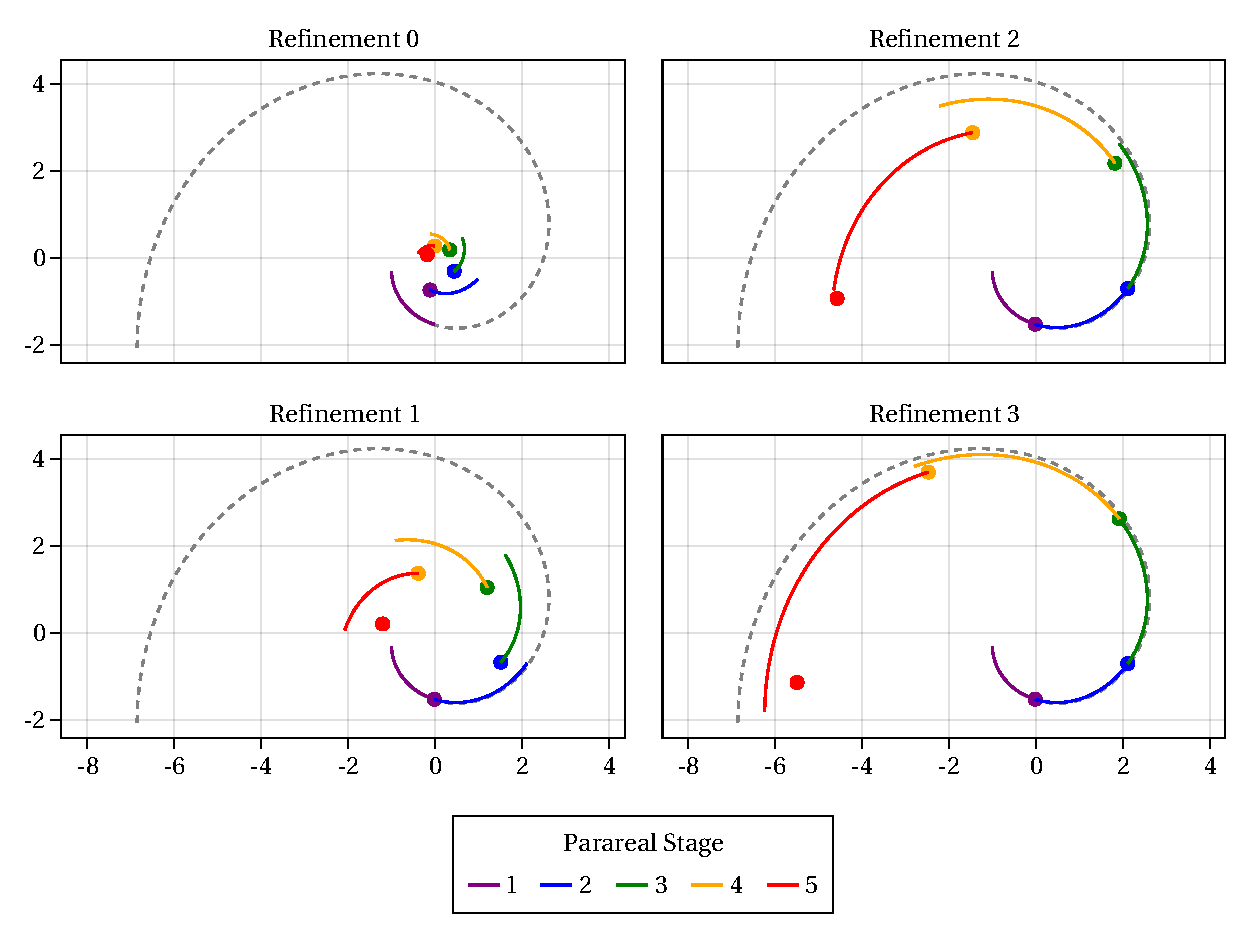
\includegraphics[width=\textwidth]{figures/fig_parareal_example.pdf}
    \caption[Parareal method applied to a linear ODE]{%
      First couple of refinements $k$ of the
      parareal method applied to the linear problem \eqref{eq:pr:linear}.
      The stages $n$ are decoded by color,
      dots denoting $U^k_n$ and lines $F(\optional{}, t_{n-1}, U^k_{n-1})$.
      The dashed gray curve represents the exact solution.
    }
    \label{fig:pr:linear}
  \end{figure}

  \autoref{fig:pr:linear} shows the first couple of iterations of the parareal method applied the problem above.
  For a fixed refinement $k$,
  the values $U^k_n \approx u(t_n)$ (represented by dots) are computed in sequence,
  \cf the horizontal traces in \autoref{fig:pr:DAG}.
  After that, the fine solutions $F(U_n^k)$ (represented by lines) can then be computed in parallel.
  The parareal method only ensures convergence of $U_n^k$.
  Therefore, before convergence is reached,
  the high-resolution trajectories are discontinues at $t_n$.
  Furthermore, note that the overall accuracy of the parareal solution is limited by the accuracy of $F$,
  which explains the remaining gap between the colored and the gray line.
\end{example}

\section{Parareal as a Multiple Shooting Method}
\label{sec:pr:newton}

The following construction is based on \citeauthor{Gander2007}~\cite{Gander2007}.
Consider again the autonomous \ac{IVP}
\begin{equation}
  \tag{\ref*{eq:IVP}}
  \left\{
  \begin{aligned}
    \dot u &= f(u) \\
    u(t_0) &= u_0
  \end{aligned}
  \right.
\end{equation}
Note that the solution $u : [t_0,t_f] \to V $ depends on the initial value $U_0$.
For a discretization $t_0 < t_1 < \ldots < t_N = t_f$
define the local problems
\begin{equation}
  \left\{
  \begin{aligned}
    \dot u_n &= f(u_n) \\
    u_n(t_n) &= U_n
  \end{aligned}
  \right.
\end{equation}
for $n \in \Set{0,\ldots,N-1}$
and determine suitable initial values $U_n$.
Watch the slight abuse of notation in $u_0$
for the initial value $u_0 \in V$
and the solution $u_0 : [t_0,t_1] \to V$ to the first local problem.
The local solutions $u_n : [t_n,t_{n+1}] \to V$ represent a global solution to the \ac{IVP}~\eqref{eq:IVP} if
\begin{equation}
  F(U_0, \ldots, U_{N-1}) :=
  \left(
  \begin{aligned}
    U_0 &- u_0 \\
    U_1 &- u_0(t_1, U_0) \\
    &\vdotswithin{-} \\
    U_{N-1} &- u_{N-2}(t_{N-1}, U_{N-2})
  \end{aligned}
  \right)
  \overset{!}{=} 0.
\end{equation}
Let $U := (U_0, \ldots, U_{N-1})$ and $\mathcal J_F(U)$ denote the Jacobian of $F$ at $U$.
Then, Newton's method reads
\begin{equation}
  U^{k+1} = U^k - \mathop{\mathcal J_F(U^k)^{-1}} F(U^k)
\end{equation}
or, equivalently, avoiding the inversion of the Jacobian,
\begin{equation}
  \begin{bmatrix}
    I \\
    -\pdiff{U_0}{u_0}(t_1, U_0) & I \\
    & \ddots & \ddots \\
    && -\pdiff{U_{N-2}}{u_{N-2}}(t_{N-1}, U_{N-2}) & I
  \end{bmatrix}
  (U^{k+1} - U^k) = -F(U^k)
\end{equation}
Writing the above in separate equations yields
\begin{equation}
  \left\{
  \begin{aligned}
    U^{k+1}_0 &= u_0 \\
    U^{k+1}_n &= u_n(t_{n+1}, U^k_n) + \pdiff{U^k_n}{u_n}(t_{n+1}, U^k_n) (U^{k+1}_n - U^k_n).
  \end{aligned}
  \right.
\end{equation}
Lastly, choosing a fine propagator $F(U^k_n) := F(t_{n+1}; t_n, U^k_n) \approx u_n(t_{n+1}, U^k_n)$,
a coarse propagator $G$ according to
\begin{equation}
  \label{eq:pr:G}
  G(U^{k+1}_n) - G(U^k_n)
  \approx
  \pdiff{U^k_n}{u_n}(t_{n+1}, U^k_n) (U^{k+1}_n - U^k_n)
\end{equation}
as well as initial values $ U^0_{n+1} = G(U^0_n) $,
reveals the parareal method of \citeauthor{Baffico2002}~\cite{Baffico2002},
\begin{equation}
  \left\{
  \begin{aligned}
    U^0_{n+1} &= G(U^0_n),
    \quad
    U^0_0 = u_0 \\
    U^{k+1}_{n+1} &= F(U^k_n) + G(U^{k+1}_n) - G(U^k_n)
    .
  \end{aligned}
  \right.
\end{equation}
A Taylor expansion of $G(U^{k+1}_n) \approx u_n(t_{n+1}, U^{k+1}_n)$ around $G(U^k_n)$ justifies Equation~\eqref{eq:pr:G}.

\section{Application to \texorpdfstring{\act{LRSIF}s}{LRSIFs}}
\label{sec:pr:DRE}

Let the \acp{LRSIF}
\begin{equation}
\begin{aligned}
  G(U^{k+1}_n) &= \mathop{L_{G,k+1}} \mathop{D_{G,k+1}} \mathop{L_{G,k+1}^\T} \\
  F(U^k_n)     &= \mathop{L_{F,k}}   \mathop{D_{F,k}}   \mathop{L_{F,k}^\T} \\
  G(U^k_n)     &= \mathop{L_{G,k}}   \mathop{D_{G,k}}   \mathop{L_{G,k}^\T}
\end{aligned}
\end{equation}
be given.
Using the low-rank update formulas described in \autoref{sec:lowrank},
the parareal update \eqref{eq:pr:method} reads
\begin{equation}
  \hat L \hat D \hat L^\T :=
  \begin{bmatrix}
    L_{G,k+1} &
    L_{F,k} &
    L_{G,k}
  \end{bmatrix}
  \begin{bmatrix}
    D_{G,k+1} \\
    & D_{F,k} \\
    && -D_{G,k}
  \end{bmatrix}
  \begin{bmatrix}
    L_{G,k+1}^\T \\
    L_{F,k}^\T \\
    L_{G,k}^\T
  \end{bmatrix}
  .
\end{equation}
Note the downdate in the last block component.
The actual low-rank representation of~$U^{k+1}_{n+1}$ is set to a column compression of~$\hat L \hat D \hat L^\T$
using \autoref{alg:lowrank:compression}.

%\section{Alternative Parallel-in-Time Solvers}

\renewcommand{\textfraction}{0.2} % default
\chapter{Implementation and Experimental Results}
\label{sec:impl}

Julia is a multi-paradigm language created by \citeauthor{Julia} at the Massachusetts Institute of Technology~(MIT)~\cite{Julia}.
While development on the language began in~2009, its version~1.0 has been released in 2018.
This chapter first covers the general properties of the two Julia packages created during the work on this thesis.
Both of these packages have an automated test suite with a coverage of well over \SI{90}{\percent}.
Lastly, the packages are applied to the Rail benchmark problem~\cite{morwiki_steel}.

\section{DifferentialRiccatiEquations.jl}
\label{sec:impl:DRE}

% Don't mention the inconsistency in tspan!  I was inspired by Norman's code,
% which received tspan sorted, i.e. in forwards time, and internally reversed
% it before and after solving.  Not knowing what I was doing, I thought
% accepting tspan in backwards time was a clever idea.  Now this package has to
% be used with backwards tspan, while having the equations stated in forwards
% time.
%
% https://gitlab.mpi-magdeburg.mpg.de/jschulze/DifferentialRiccatiEquations.jl/-/issues/6#note_13652

This package is concerned with sequential \ac{DRE} solvers only.
The general user interface has been inspired by \code{DifferentialEquations.jl}~\cite{DifferentialEquations},
and looks like this:
\begin{lstlisting}[
  caption={[User interface of \code{DifferentialRiccatiEquations.jl}]},
]
prob = GDREProblem(E, A, B, C, X0, tspan)
alg = Ros1()
sol = solve(prob, alg; dt=dt)
\end{lstlisting}
Besides \julia{Ros1()} and \julia{Ros2()},
which correspond to the algorithms described in \autoref{sec:ros},
there also is a \julia{Ros4()} solver.
It is based on \citeauthor{Lang2017}~\cite[Appendix~A]{Lang2017} and only supports the dense case.
The \julia{GDREProblem} type is parametrized on the type of the initial value \julia{X0},
by which the proper \ac{ALE} solver is selected via runtime dispatch on \julia{solve()}.
Dense initial values are represented by the built-in \julia{Matrix} type,\footnote{%
  \url{https://docs.julialang.org/en/v1.6/stdlib/LinearAlgebra/}}
and lead to a direct \ac{ALE} solver from \code{MatrixEquations.jl}~\cite{MatrixEquations}.
Initial values in \ac{LRSIF} are represented by the new \julia{\LDLt} type,
and lead to the iterative \ac{ADI} solver described in \autoref{sec:ADI}.

\paragraph{Representation of Low-Rank Matrices}

Suppose $X = LDL^\T$ and \julia{X = \LDLt(L, D)} are mathematical and Julia representations of the same objects,
$L\in\R^{n\times r}$, $D\in\R^{r\times r}$.
Then, the internal representation of~\julia{X} consists of lists~\julia{[L]} and~\julia{[D]},
such that updates may be performed lazily by merely collecting all the summands,
\cf \autoref{sec:lowrank}.
Compression of~\julia{X} is performed once these lists contain 10 elements or more,
or if the equivalent inner dimension is too large, $r \geq \onehalf n$.
This causes a compression every 10 iterations of the \ac{ADI} or earlier.
This is not configurable yet,
\cf~\autoref{lst:impl:LDLt}.
Note that line~\ref{line:impl:LDLt:compression_due} mainly guards the situation
when a user accesses $L$ and $D$ (via iteration: \mbox{\julia{L, D = X}}),
compression is not performed twice.
All internal usages guarantee the assumption in the comment above line~\ref{line:impl:LDLt:compression_due}.

\begin{lstlisting}[
  float=tp,
  caption={%
    [{Definition of \julia{\LDLt} and \julia{(+)}}]
    Definition of \julia{\LDLt} and addition \julia{(+)} of \ac{LRSIF} objects.
    The compression, \julia{compress!()}, is described in \autoref{alg:lowrank:compression}.
  },
  label={lst:impl:LDLt},
  escapechar=\%,
]
struct %\LDLt%{TL,TD}
    Ls::Vector{TL}
    Ds::Vector{TD}
end

function Base.:(+)(Xs::%\LDLt%{TL,TD}...) where {TL,TD}
    Ls = TL[]
    Ds = TD[]
    for X in Xs
        append!(Ls, X.Ls)
        append!(Ds, X.Ds)
    end
    X = %\LDLt%{TL,TD}(Ls, Ds)
    maybe_compress!(X)
end

function compression_due(X::%\LDLt%)
    # If there is only one component, it has likely already been compressed:
    length(X.Ls) == 1 && return false%\label{line:impl:LDLt:compression_due}%
    # Compression is due every couple of modifications:
    length(X.Ls) >= 10 && return true
    # Compression is due if rank is too large:
    n = size(X, 1)
    r = rank(X)
    return r >= 0.5n
end

function maybe_compress!(X::%\LDLt%)
    compression_due(X) || return X
    compress!(X)
end
\end{lstlisting}

\paragraph{Representation of Shifted Matrices}

Recall that the Rosenbrock methods yield \acp{ALE},
whose system matrices are sparse matrices shifted by a low-rank matrix,
\cf $\tilde A_n$ in \autoref{alg:ros1:smw} of \autoref{alg:ros1} and $\hat A_n$ in \autoref{alg:ros2:smw} of \autoref{alg:ros2}.
Within the \ac{ADI}, these matrices are updated by another sparse matrix,
\cf $A^+_k$ in \autoref{alg:ADI:smw} of \autoref{alg:ADI}.
Overall, taking \Ros{1} as an example,
the system to be solved with is
\begin{equation}
  A_k^+ =
  \big(\big( A_n - \tfrac{1}{2\tau} E \big)^\T + \alpha_k E \big) - K_n^\T B^\T
  .
\end{equation}
This structure, however, is completely hidden from the \ac{ADI} code via
\begin{lstlisting}[
  caption={[Abstraction of shifted linear system between Rosenbrock method and ADI]},
  %caption={Representation of shifted linear systems},
  escapechar=\%,
]
%\~A% = LowRankUpdate(A - E/(2%$\tau$%), -1, B, K)
R = %\LDLt%(G, S)
lyap = GALEProblem(E, %\~A%, R)
solve(lyap, ADI())
\end{lstlisting}
Thereby, the \ac{ADI} transposes $\tilde A$ via \julia{adjoint()},
%\footnote{%
%  In Julia, \julia{A'} is syntactic sugar for \julia{adjoint(A)},
%  \cf \url{https://docs.julialang.org/en/v1.6/manual/functions/\#Operators-With-Special-Names}
%}
and adds the sparse $\alpha_k E$ via \julia{(+)} without losing the \julia{LowRankUpdate} structure.
Its main feature, however, is solving the corresponding linear system via the backslash operator~\julia{(\textbackslash)}
using the Sherman-Morrison-Woodbury formula,
\cf \autoref{sec:basics:smw}.
See \autoref{lst:impl:LowRankUpdate} for the basic definition of \julia{LowRankUpdate} and the aforementioned functions.

\def\mi{\textsuperscript{-1}}
\def\ma{\protect\makebox[\widthof{a}]{$\alpha$}}
\begin{lstlisting}[
  float=tp,
  caption={%
    [{Definition of \julia{LowRankUpdate} as well as \julia{(+)} and \julia{(\textbackslash)}}]
    Definition of \julia{LowRankUpdate},
    a lazy representation of the shifted linear system $A + \alpha^{-1} UV$,
    as well as addition \julia{(+)} of a sparse matrix,
    and left-division \julia{(\textbackslash)}
    using the Sherman-Morrison-Woodbury formula,
    \cf \autoref{sec:basics:smw}.
  },
  label={lst:impl:LowRankUpdate},
  escapechar=\%,
]
struct LowRankUpdate{TA,T,TU,TV}
    A::TA
    %\ma%::T
    U::TU
    V::TV
end

function Base.adjoint(AUV::LowRankUpdate)
    A, %\ma%, U, V = AUV
    LowRankUpdate(A', %\ma%', V', U')
end

function Base.:(+)(AUV::LowRankUpdate, E::AbstractMatrix)
    @assert issparse(E)
    A, %\ma%, U, V = AUV
    LowRankUpdate(A+E, %\ma%, U, V)
end

function Base.:(\)(AUV::LowRankUpdate, B::AbstractVecOrMat)
    A, %\ma%, U, V = AUV

    FA = factorize(A)
    A%\mi%B = FA \ B
    A%\mi%U = FA \ U

    S = %\ma% * I + V * A%\mi%U
    S%\mi%VA%\mi%B = S \ (V * A%\mi%B)

    X = A%\mi%B - A%\mi%U * S%\mi%VA%\mi%B
    return X
end
\end{lstlisting}

% Above listing used to contain `_factorize`, which is a custom implementation.
% It's only purpose was to ensure that if the factorization is a `Diagonal`,
% its diagonal is a dense vector. In some of my dummy experiments, this was
% faster to solve with. However, A and E are basically never diagonal, so this
% function exists for "historical reasons" (TM) only.


\section{ParaReal.jl}

This section describes the general properties of the \julia{ParaReal.jl} package.
It has been designed with the following requirements in mind:
\begin{enumerate}
  \item\label{item:impl:goal:schedule}
    Schedule each stage on a separate process.

    This is a sensible default for the application at hand,
    which is memory bound for typical problem sizes.
    Yet, the scheduling strategy should be modifiable/extendable.
  \item\label{item:impl:goal:variablesize}
    Allow the data transferred be variable in size.

    This is necessary to transmit \ac{LRSIF} of varying rank and, therefore, storage size depending on $n$ (and $k$).
  \item\label{item:impl:goal:notransfer}
    Do not transfer the final solution data back to the calling/managing process.

    For fine resolutions, the storage requirements are immense.
    The overall solution might not fit in memory of a single compute node.
    Therefore, it has to be possible that each stage $n$ saves its local (fine) solution along $[t_{n-1},t_n]$ directly to disk,
    without sending it to the calling process first.
\end{enumerate}
On top of that:
\begin{enumerate}[resume]
  \item\label{item:impl:goal:modularity}
    The parareal implementation has to be modular,
    \ie easy to use/adapt for other problems than \ac{LRSIF} formulations of \ac{DRE}.
\end{enumerate}

Requirement \ref{item:impl:goal:schedule} is achieved by the abstract type \julia{Schedule},
whose sole subtype (for now) is \julia{ProcessesSchedule}.
It takes a list of $N$ worker/process ids, each of which will execute one stage.
Future strategies may be implemented by defining new subtype of \julia{Schedule}, \eg
\julia{ThreadsSchedule} using threads on a single process,
\julia{HybridSchedule} which uses both threads and processes, and
\julia{DaggerSchedule} which uses the abstractions provided by \julia{Dagger.jl}.\footnote{\url{https://github.com/JuliaParallel/Dagger.jl}}

Requirement \ref{item:impl:goal:variablesize} is trivial to fulfill using Julia's \julia{RemoteChannel} data type.
Requirement \ref{item:impl:goal:modularity} imposes a non-specific naming scheme for
user interface functions and the name of the unknown,
as to not clash with the standard nomenclatures of other disciplines.\footnote{%
  For example,
  many parareal papers use $U$ to name the unknown,
  many matrix \ac{ODE} papers use $X$,
  and the widely-used \julia{DifferentialEquations.jl} package~\cite{DifferentialEquations} uses $u$.
}
The next section will describe the user interface of the \julia{ParaReal.jl} package,
and how to cope with problem~\ref{item:impl:goal:notransfer}.

\subsection{User Interface}

In applications one is usually interested in a high temporal resolution,
while the parareal method is only used to obtain \enquote{fast} convergence.
Therefore, the \julia{ParaReal.jl} package distinguishes between a local solution along $[t_{n-1}, t_n]$ and the final value of which,
\begin{align*}
  F(U_{n-1}^k) &= \julia{value(fsolve(prob))} \\
  G(U_{n-1}^k) &= \julia{value(csolve(prob))}
\end{align*}
where \julia{prob} is an instance of the global \ac{IVP}~\eqref{eq:IVP}
restricted to the local time slice~$[t_{n-1}, t_n]$ and initial value~$U_{n-1}^k$.
The actual solver functions \julia{csolve} (\enquote{coarse}) and \julia{fsolve} (\enquote{fine})
are provided as arguments to \julia{ParaReal.Algorithm()}.
In order to support custom \ac{IVP} types,
a user has to defined methods for \julia{initial\_value()} to extract the global initial value $U_0$,
and \julia{remake\_prob()} to adjust the global problem for the local time slice and initial value.
For more details, refer to the documentation of the respective functions available from within Julia.

In order to support new solution types,
a custom implementation of the parareal update formula~\eqref{eq:pr:method} may be needed.
This can be specified as an optional third argument to \julia{ParaReal.Algorithm}.
The default is \julia{ParaReal.default\_update!()},
whose implementation is given in~\autoref{lst:impl:default_update!}.
Adding methods to \julia{default\_update!()} is not recommended.
Any custom implementation of the parareal update formula must follow the interface of \julia{default\_update!()}.

\def\sk{\textsuperscript{k}}
\def\skmi{\textsuperscript{k-1}}
\lstinputlisting[%
  float=t,
  label={lst:impl:default_update!},
  caption={Default implementations of the parareal update formula},
  escapechar=\%,
  breaklines=true,
]{code/default_update.jl}
% The form a+b+(-c) is for historical reasons. The LDLt data structure used to eagerly concatenate the
% matrices instead of collecting them lazily, as it does now. Back then, using a ternary plus meant
% fewer allocations (then: 2 allocs for L and 2 allocs for D, now: 0 allocs for L and 1 alloc for D)
% before compression.

The remainder of this section is devoted to a complete example of a user-defined problem type ($N=3$, $K=2$).
The problem type will be a mere placeholder that forwards its initial value,
while the solver functions will count the applications of $F$ and $G$ a particular solution is composed of.
Start by launching some worker processes and loading the necessary packages:
\lstinputlisting[%
  caption={User-defined problem type for \julia{ParaReal.jl}},
  label={lst:impl:parareal_counting},
  lastline=4,
]{code/parareal_counting.jl}
Next, define the problem type and ensure that definition is available on all processes.
The only requirement to the problem type is to have a \julia{tspan} field.\footnote{%
  Alternatively, it must support \julia{getproperty(prob, :tspan)}.
}
In the context of \ac{ODE}, this should not clash with any other notation.
\addtocounter{lstnumber}{1} %FIXME
\lstinputlisting[nolol, firstnumber=last, linerange=problem-end]{code/parareal_counting.jl}
The solution type will hold counters of the applications of $F$ and $G$:
\lstinputlisting[nolol, firstnumber=last, linerange=solution-end]{code/parareal_counting.jl}
Define the solver functions and problem instance and execute the parareal pipeline.
The solver functions are defined as closures,
such that they can be serialized and transferred to the worker processes.
Note that this code is only executed on the managing process:
\lstinputlisting[nolol, firstnumber=last, linerange=solve-end]{code/parareal_counting.jl}
Lastly, extracting the final values $U_1^1$, $U_2^2$, and $U_3^2$ via
\lstinputlisting[nolol, firstnumber=last, linerange=result-end]{code/parareal_counting.jl}
yields:
\begin{align*}
  &\julia{Counters(1,0)}, \text{ since} &
  U_1^1 &= F(U_0) \\
  &\julia{Counters(2,0)}, \text{ since} &
  U_2^2 &= F(F(U_0)) \\
  &\julia{Counters(3+2+2,2+4+4)}, \text{ since} &
  U_3^2 &= G(F(F(U_0))) + F(U_2^1) - G(U_2^1) \\
  && U_2^1 &= G(F(U_0)) + F(G(U_0)) - G(G(U_0))
\end{align*}

The full trajectory of the fine solver may be extracted using \julia{ParaReal.solution()}.
However, solution and value are identical in the example above,
\cf line~\ref{line:impl:parareal_counting:value}.
\autoref{lst:impl:store} shows the recommended pattern of
storing the fine solutions directly from the worker processes
via \julia{ParaReal.fetch\_from\_owner()}.

\lstinputlisting[%
  float=tpb, % TODO: ensure this doesn't disrupt the inline code snippets
  caption={%
    [Store fine parareal solutions directly from the worker processes]
    Store fine parareal solutions directly from the worker processes.
    This works well as a blueprint for \julia{DrWatson.\_wsave(dir, sol)} \cite{DrWatson}.
  },
  label={lst:impl:store},
]{code/parareal_store.jl}

\subsection{JIT Compilation and Warm-Up}

Julia is a \ac{JIT} compiled language~\cite{Julia},
which means that code is compiled just before it is first executed,
unless it has already been compiled.
Therefore, unless the code has been compiled \ac{AOT},
only the second execution of code is fast.
This effect is called \emph{warm-up}.
As mentioned in~\autoref{sec:pr}, computing the coarse solutions
$G(U_n^*)$ is essentially a sequential operation over all $n$.
The computations of $F(U^*_n)$ can only be parallelized after such a global coarse solve.
Therefore, it is critical that the individual coarse solutions are available as fast as possible.

In order to describe the runtime of the present parareal implementation,
let $t_F$, $t_G$ denote the runtime of $F$ and $G$, respectively.
Let $N$ be the number of stages $1 \leq n \leq N$,
and $K$ be the number of refinements $0 \leq k \leq K$.
Let $\trampup$ be the overhead imposed on each computing the first coarse solution $G(U_n^0)$,
and $\twarmup$ be a general global overhead.
Further, we make the following assumptions:
\begin{enumerate}
  \item
    $t_F$ and $t_G$ are constant, \ie do not depend on $n, k$.
  \item
    \label{item:impl:assumption:tU}
    The time to compute the actual value $U_n^k$ is negligible,
    \cf~\autoref{lst:impl:default_update!}.
  \item
    The overhead to check for convergence is negligible.
  \item
    Communication time is negligible.
  \item
    All stages $n$ compute $K$ refinements, \ie $k_n = K \enspace\forall n$.
\end{enumerate}
The runtime may then be estimated using
\begin{equation}
\label{eq:impl:tpar}
  \hattpar
  = \twarmup
  + \underbrace{
    \strut
    N \cdot (\trampup + t_G)
  }_{\substack{
    \text{stages $1\leq n\leq N$}\\
    \text{refinement $k=0$}
  }}
  + \underbrace{
    \strut
    K \cdot (t_F + t_G)
  }_{\substack{
    \vphantom{\text{stage}}
    n = N \\
    1 \leq k \leq K
  }}
  + t_F
\end{equation}
where the final $t_F$ is to compute the best fine solution available.
These assumptions are compatible to the generic timeline \autoref{fig:timeline:generic}.
As will be described later,
\begin{equation}
  \twarmup + \trampup
  = t_{\JIT(G)} + t_\text{other}
\end{equation}
\ie the goal is to offset/reduce the ramp-up delay $\trampup$
at the cost of a one-time overhead $\twarmup$.
$t_{\JIT(G)}$ denotes the compile time of $G$.
Refer to \autoref{tab:impl:warmup} for the measurements corresponding to \autoref{fig:impl:warmup}.

\begin{figure}[p]
  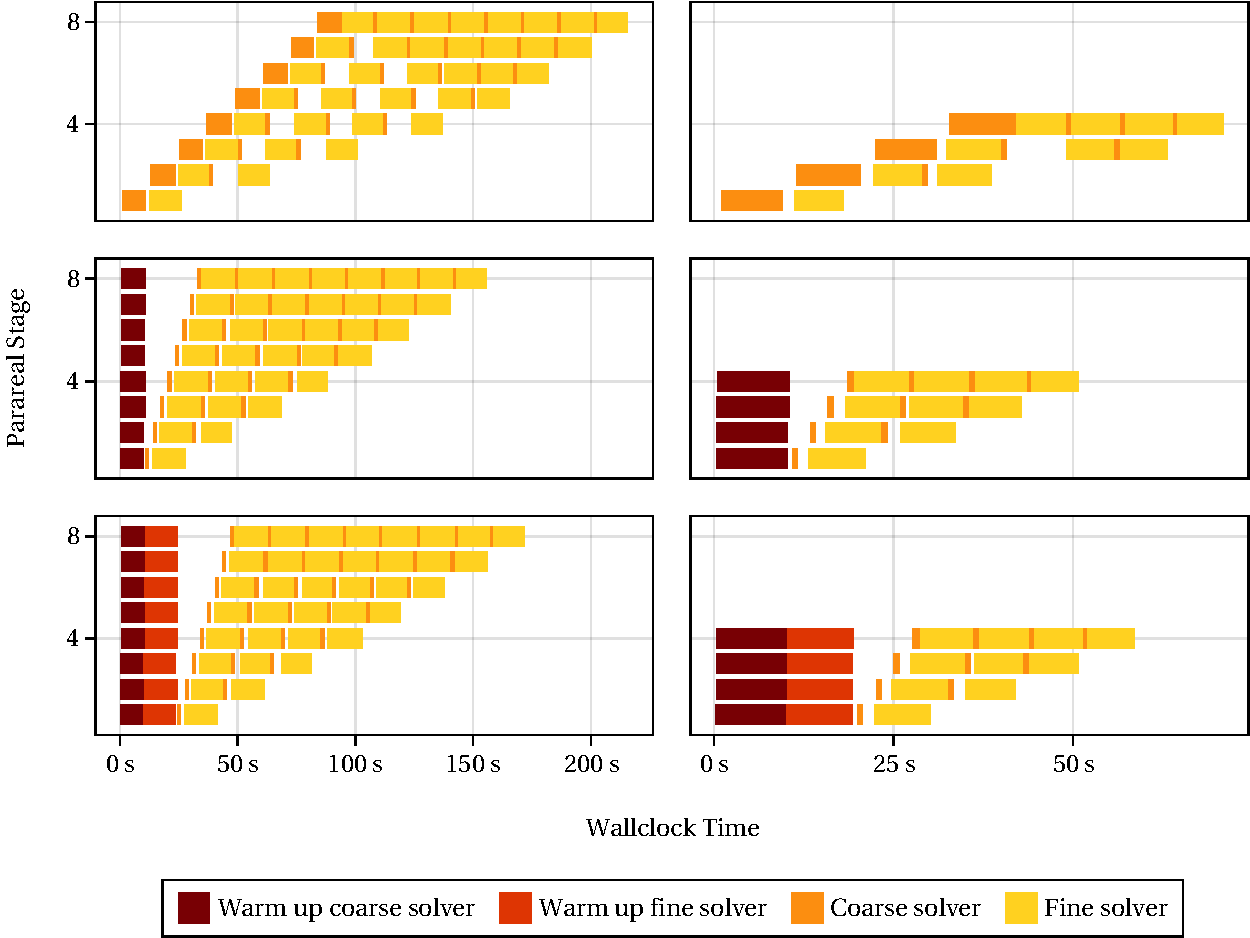
\includegraphics[width=\textwidth]{figures/fig_impl_warmup2.pdf}
  \caption[Timeline diagrams comparing the effect of JIT compiler warm-up]{%
    Timeline diagrams comparing the effect of \acs{JIT} compiler warm-up.
    Left: $N=8$ processes running on two compute nodes,
    right: $N=4$ processes running on a laptop.
    Top: no warm-up,
    middle: warming up coarse solver $G$ (\julia{csolve}),
    bottom: warming up coarse and fine solver $F$ (\julia{fsolve}).
  }
  \label{fig:impl:warmup}
\end{figure}

\begin{table}[p]
  \centering
  \begin{tabular}{lccccccc}
    \toprule
    warm-up & $N$ & $\twarmup$ & $\trampup$ & $t_G$ & $t_F$ & $\tpar$ & $\hattpar$ \\
    \midrule
    none  & 8 \\
    $G$   & 8 \\
    $G,F$ & 8 \\
    \midrule
    none  & 4 \\
    $G$   & 4 \\
    $G,F$ & 4 \\
    \bottomrule
  \end{tabular}
  \caption[Measurements corresponding to \autoref*{fig:impl:warmup}]{%
    Measurements corresponding to \autoref*{fig:impl:warmup}
    based on~\eqref{eq:impl:tpar}.
    The actual runtime is denoted by $\tpar$.
    $t_F$ and $t_G$ are estimated as the median,
    $\twarmup$ as the maximum of their respective runtimes.
    $\trampup$ is taken as the mean delay between adjacent $G(U_n^0)$.
    All timings are in seconds.
  }
  \label{tab:impl:warmup}
\end{table}

\paragraph{Sequential \ac{JIT} compilation}

Without any precautions,
\begin{equation*}
  \twarmup = 0,
\end{equation*}
\ac{JIT} compilation of $G$ happens sequentially,
as computing $G(U_n^k)$ is essentially sequential over $n$.
This effect is especially severe if the executors of different parareal iterations $(n,k)$ do not share the results of code compilation.
These executors may be processes, threads~(pthreads), or tasks~(green threads).
For the present implementation,
there is a one-to-one mapping between processes and stages $n$,
which means the compilation happens exactly once per stage $n$ and is reused between refinements $k$.\footnote{%
  As of the writing of this thesis, Julia does not reuse code compiled between processes.
}
This is visible in the first row of \autoref{fig:impl:warmup}
by the first occurrences of $G$ for each stage $n$,
which marks the computation of $G(U_n^0)$,
whose execution time includes compilation time.
Therefore, the first occurrences of $G$ take substantially longer than the subsequent ones.
The computation of the parareal update has a negligible duration,
and is therefore not shown in the timeline plot,
\cf assumption~\ref{item:impl:assumption:tU}.

\paragraph{Parallel \acs{AOT} compilation}

Since \julia{ParaReal.jl} is independent of $F$ and $G$ as well as the actual data type of the underlying \ac{IVP},
full \ac{AOT} compilation is difficult, and has to be done by users of the package.
A more naive approach is to manually warm up critical parts of the code by executing them before they are actually needed.
In the context of \julia{ParaReal.jl},
doing so allows to perform the compilation in parallel,
which significantly decreases the time to compute all coarse solutions $G(U_n^*)$.
This is visible in the middle and bottom rows of \autoref{fig:impl:warmup},
where
\begin{align*}
  \twarmup &= t_{\JIT(G)} + t_G
  \enspace
  \text{and} \\
  \twarmup &= t_{\JIT(G)} + t_G + t_{\JIT(F)} + t_F,
\end{align*}
respectively.
Warming up both $F$ and $G$ has (as expected) a negligible effect on~$\trampup$,
while adding a major overhead to~$\hattpar$ as generally $t_F \gg t_G$.

\paragraph{Precompilation}

Besides reducing the delay of executing $F$ and $G$,
it is also important to reduce the delay of any code from \julia{ParaReal.jl} that doesn't depend on them.
The package is merely responsible for orchestrating the execution of the parareal iterations $(n,k)$.
Therefore, the delay of the first execution of \julia{ParaReal.jl} code is dominated by type inference.\footnote{%
  At least it likely is. Taking measurements is highly non-trivial and out of the scope of this thesis.
  For more details see: \url{https://julialang.org/blog/2020/08/invalidations/}
}
The time spent on type inference can be minimized by precompilation,
which happens when the package is first loaded,
and whose results are cached and reused when the package is loaded again.
Exploiting this is highly non-trivial and out of the scope of this thesis.\footnote{\url{https://julialang.org/blog/2021/01/precompile_tutorial/}}

\todo[inline]{%
How to cite these webpages properly?
Should I do anything about the speculation in the paragraph, or the exposure of which in the footnote?
}

\paragraph{Summary}

\todo[inline]{
  Relate \autoref{fig:impl:warmup} and \autoref{fig:timeline:revised}:
  $k=K$ and thus early convergence not visible.
  $n+K\geq N$ most pronounced in top left diagram.
}

In the case of no warm-up, $\twarmup=0$, the overall compilation overhead caused by $G$ scales linearly in $N$.
If $G$ is instead being warmed up, $\twarmup=t_{\JIT(G)}$, that overhead depends only on the underlying problem.
However, the remaining $t_\text{other}$ includes compilation time for communications,
\eg to serialize the data types representing $U_n^k$,
and to establish a connection between adjacent pipeline stages.\footnote{%
  By default, connections between processes are established when they are first used.
  Here, only the connections between the calling process and the worker processes,
  each executing a pipeline stage,
  have been created.
}
This still leaves a linear overhead in the number of stages $N$.
Furthermore, due to the one-to-one mapping between stages $n$ and processes,
some processes will finish earlier than others.
This leaves potential to better utilize given hardware.

\subsection{Lack of Asynchronous Data Transfer}
\label{sec:impl:pr:sync}

A common strategy to improve CPU utilization is to perform data transfers between processes asynchronously.
Julia offers the \julia{RemoteChannel} data structure for this purpose.
As of the writing of this thesis,
the \julia{RemoteChannel} is not thread-safe.\footnote{\url{https://github.com/JuliaLang/julia/issues/37706}}
More specifically, it must be used from thread~1 of each process.
This means that in order to asynchronously send the interface~values~$U_n^{k+1}$ from stage $n$ to the next,
one would have to move the calls to~$F$ and~$G$ off of thread~1.
The reason is that many implementations of $F$ and $G$ don't have an implicit (cooperative) yield point to Julia's runtime,
such that no task can run asynchronously on thread~1 next to the task executing~$F$ and~$G$.
This is particularly true for code that doesn't require~\ac{IO},
\eg for many methods from Julia's \julia{LinearAlgebra} standard library,
which internally call \code{LAPACK}.

\todo{Mention that Julia runs single-threaded as to not oversaturate machine? BLAS/LAPACK launch their own threads.}
The solution described in the previous paragraph is not yet implemented,
\ie all data transfers are synchronous.
This causes gaps visible in \autoref{fig:impl:warmup} after $G$ and before $F$,
whose ends roughly align with the beginnings of calls to $G$ on the next stage.

Another effect is that the iterations $(n,k)$ for which $n+k \geq N$ do not show this gap.
The reason is twofold.
The last stage $N$ doesn't need to send any data, therefore has no \ac{JIT} warm-up delay for the first iteration $k=0$ and no gap in the diagram.
This causes the next refinement $k=1$ of the previous stage $N-1$ to have a noticeably smaller gap,
since its transmission code has already been compiled.
This effect propagates back-to-front through the still running pipeline stages.

The exact size of the gap between the computations of $G(U_{n-1}^k)$ and $F(U_{n-1}^k)$ of stage $n$ is determined by
\begin{enumerate}
  \item\label{item:impl:gapsize:1}
    the execution time of the transfer of $U_n^k$ to stage $n+1$, and
  \item\label{item:impl:gapsize:2}
    the overhead included in the computation of $G(U_n^{k-1})$,
    \ie the previous iterate $k-1$ on the next stage $n+1$.
\end{enumerate}
For $k=0$, \ref{item:impl:gapsize:2} is zero.
For $k=1$ and no warm-up, \ref{item:impl:gapsize:2} includes compilation time and dominates \ref{item:impl:gapsize:1},
which shadows the effect described in the previous paragraph for the first row of \autoref{fig:impl:warmup}.
For $k\geq 2$, \ref{item:impl:gapsize:2} is essentially zero.\footnote{%
  If due to user code the data types of $U_n^*$ changes, recompilation might be necessary.
}

\subsection{Early Convergence}
\label{sec:impl:pr:conv}

Also considering \autoref{thm:pr:conv}, ...

To summarize, the revised timeline plot is shown in \autoref{fig:timeline:revised},
\cf~\autoref{fig:timeline:generic}.

\begin{figure}[t]
  \centering
  \begin{tikzpicture}
  \def\myscale{0.6}
  % axis and labels
  \node[below] at (5,-0.5*\myscale-0.3) {\footnotesize Wallclock Time};
  \node[rotate=90, above] at (-0.5-0.3,5*\myscale) {\footnotesize Parareal Stage};
\begin{scope}[yscale=\myscale]
  \draw[semithick] (-0.5,-0.5) rectangle (10.5,10.5);
  % timeline diagram
  \draw[thick] (0,0) rectangle node[rotate=90] {warm-up} (1,10);
  \draw[thick] (1.1,0)
    -- node[right] {$k=0$} (3.1,10)
    -- node[below] {$n=N$} (9,10)
    -- (7.4,2)
    -- node[below] {$n=k$} cycle;
  \node[right] at (8,5) {$k=K$};
  % lack of asynchronous data transfer
  \draw[thick,gray,dotted] (8.25,6.25)
    -- node[black,left] {$n+K \geq N$} (8.5,10);
  % early convergence due to "delta k = 1"
  \draw[thick,gray,dashed] (7.5,2.5)
    -- node[black,left] {convergence} (6,10);
\end{scope}
\end{tikzpicture}

  \caption[Revised schematic timeline diagram]{%
    Revised schematic timeline diagram of \julia{ParaReal.jl} implementation for $N$ stages and $K$ refinements.
    The dotted line is due to the lack of asynchronous data transfer for $n+k \geq N$,
    \cf~\autoref{sec:impl:pr:sync}.
    The dashed line indicates early convergence for $k_n < k_{n+1}$,
    \cf~\autoref{sec:impl:pr:conv}.
  }
  \label{fig:timeline:revised}
\end{figure}

\subsection{Advanced Scheduling Strategies}

\begin{itemize}
  \item
    Early stages $n=0,1,2$ become idle even before later stages receive their first $U^0_n$.
    Maybe they could be reused: measure runtime of $F$ and $G$ to compute optimum number $N$ for given number of processors.
    Alternatively, one could adjust the local time slices, \cf \url{https://gitlab.mpi-magdeburg.mpg.de/jschulze/ParaReal.jl/-/issues/2}
  \item
    If $X$ trajectories shall not be saved, solving the \ac{DRE} isn't that memory heavy.
    Creating a connection between workers in a cluster shouldn't be that expensive (they are initialized lazily, but cost should pay off).
    It might be worth it to send $U^{k+1}_n$ as well as $G(U^k_n)$ and $F(U^k_n)$ over the network in order to recycle processors.
    However, this requires a lazy DAG scheduling like \texttt{DAGGER.jl}.
  \item
    \cite[493]{Nielsen2018} relevant?
  \item
    Distributed processes vs local threads vs GPU?
\end{itemize}

\subsection{Parallel Programming Pitfalls}

\begin{itemize}
  \item
    \julia{@sync} may block\footnote{\url{https://github.com/JuliaLang/julia/issues/32677}}
    There is an experimental eager version,\footnote{\url{https://github.com/JuliaLang/julia/pull/34198}} but it doesn't support cancellation.
    In general, as of the time of writing this thesis,
    there is no recommended way to handle cancellation using the standard library,
    especially (and frustratingly) in a distributed environment.
  \item
    By default, unhandled concurrent errors are transient.\footnote{%
      \url{https://github.com/JuliaLang/julia/issues/10405}}
    That means that if a background task fails, not only does the program keep running, it doesn't even print an error.\footnote{%
      \url{https://github.com/JuliaLang/julia/pull/27722}}
    It is not easy to let unhandled concurrent errors crash the whole program.
    More severly, in a distributed environment, a failed task on one machine may easily cause a different machine to deadlock,
    \cf the previous paragraph.
    It is the user's (or the library developer's) responsibility to make errors observable,\footnote{%
      \url{https://github.com/JuliaLang/julia/pull/39518}}
    and to make sure that whole computation is properly cancelled.
  \item
    \url{https://github.com/JuliaLang/julia/issues/38931},
    \url{https://github.com/JuliaLang/julia/pull/44671}
\end{itemize}

\subsection{Where should I put this?}

\begin{itemize}
  \item
    Due to \autoref{thm:basics:dre-limit-are},
    I expect later parareal stages to require fewer Newton refinements to reach convergence.
    Therefore, each stage $n$ may defer the computation of a refinement $k$,
    until the previous stage $n-1$ finished computing its refinement $k+1$.
    That is, the number of refinements computed may differ by at most one from stage to stage.

    This effect is visible in the timeline diagram of \eg the reference solution of \autoref{fig:results:parareal:rail}.
\end{itemize}


\section{Numerical Results}

This section summarizes the results of applying the aforementioned methods to
the Rail benchmark~\cite{morwiki_steel} of size $n=371$
described in \eg~\autoref{thm:rail:parameters}.
Note that the algorithms are formulated for the problem stated in forwards time,
\begin{equation}
\left\{
\begin{aligned}
  E^\T \dot X E &= C^\T C + A^\T X E + E^\T X A - E^\T X BB^\T X E \\
  E^\T X(t_0) E &= \tfrac{1}{100} C^\T C
\end{aligned}
\right.
\end{equation}
but it's common practice to plot results in the time corresponding to the underlying \ac{OCP},
\ie $E^\T \tilde X(t_f) E = C^\T C/100$.

As described in \autoref{sec:HJT},
one is mainly interested in the accuracy of the feedback matrix
$
  K := B^\T X E \in \R^{7 \times n}
$.
For this purpose, the trajectory $K_{1,77}$ is characteristic due to its relatively large amplitude~\cite{Lang2015}.
Furthermore, the (global) relative error
\begin{equation}
\label{eq:results:err:ref}
  \frac{\norm{K(t) - K_\text{ref}(t)}_F}{\norm{K_\text{ref}(t)}_F}
\end{equation}
is analyzed \wrt a reference solution computed with the dense 4th order method described in \cite[Appendix~A]{Lang2017}.
Any error at $t=\SI{45}{\second}$ is not shown,
as it is zero due to the boundary condition of the \ac{DRE},
which would distort the overall diagram.

The tolerances for both the \ac{ADI} and parareal method,
\cf~\eqref{eq:adi:lrstop} in \autoref{sec:adi:lrstop}
and~\eqref{eq:impl:pr:conv} in \autoref{sec:impl:pr:conv},
are chosen to be $\epsilon := n\umach$
where $\umach$ denotes machine precision
and $n=371$ refers to the problem dimension.
The \ac{ADI} may perform up to 100 iterations.
A \ac{LRSIF} is compressed every 10 iterations or earlier,
if the inner dimension~$r$ reaches~$\onehalf n$,
\cf~\autoref{sec:impl:DRE}.
Furthermore, each of the $N = 450$ parareal stages requires two successive refinements without significant change
for (local) convergence,
while computing at most $K = 10$ refinements.

\begin{remark}
  In this subsection,
  $n$ may denote the problem dimension $X \in\Rnn$,
  or the time stop $t_n$,
  which is also related to the parareal stage $n$ corresponding to the time span $[t_{n-1}, t_n]$
  where $1 \leq n \leq N$.
  Furthermore,
  $K$ may denote the feedback matrix \mbox{$K = B^\T X E$},
  or the maximum number of parareal refinements $k_n \leq K$ computed per stage $n$.
  The particular meaning should be clear from its context.
\end{remark}

\subsection{Sequential Solvers}

\autoref{fig:results:sequential:rail} shows the results of the Rosenbrock schemes described in \autoref{sec:ros},
both in a dense and a \ac{LRSIF} formulation.
The low-rank variants are expected to perform identically to their dense counterparts,
which for \Ros{1} is ok.
However, there is a small difference between the second order methods for $t\leq\SI{44}{\second}$,
which destroys the order of \ac{LRSIF}~2 for about $t\leq\SI{35}{\second}$.
The general downward trend of the errors as $t$ approaches \SI{0}{\second} is due to the L-stability of the methods and the constant limit,
\cf~\autoref{thm:basics:dre-limit-are:backwards}.

\begin{figure}[tp]
  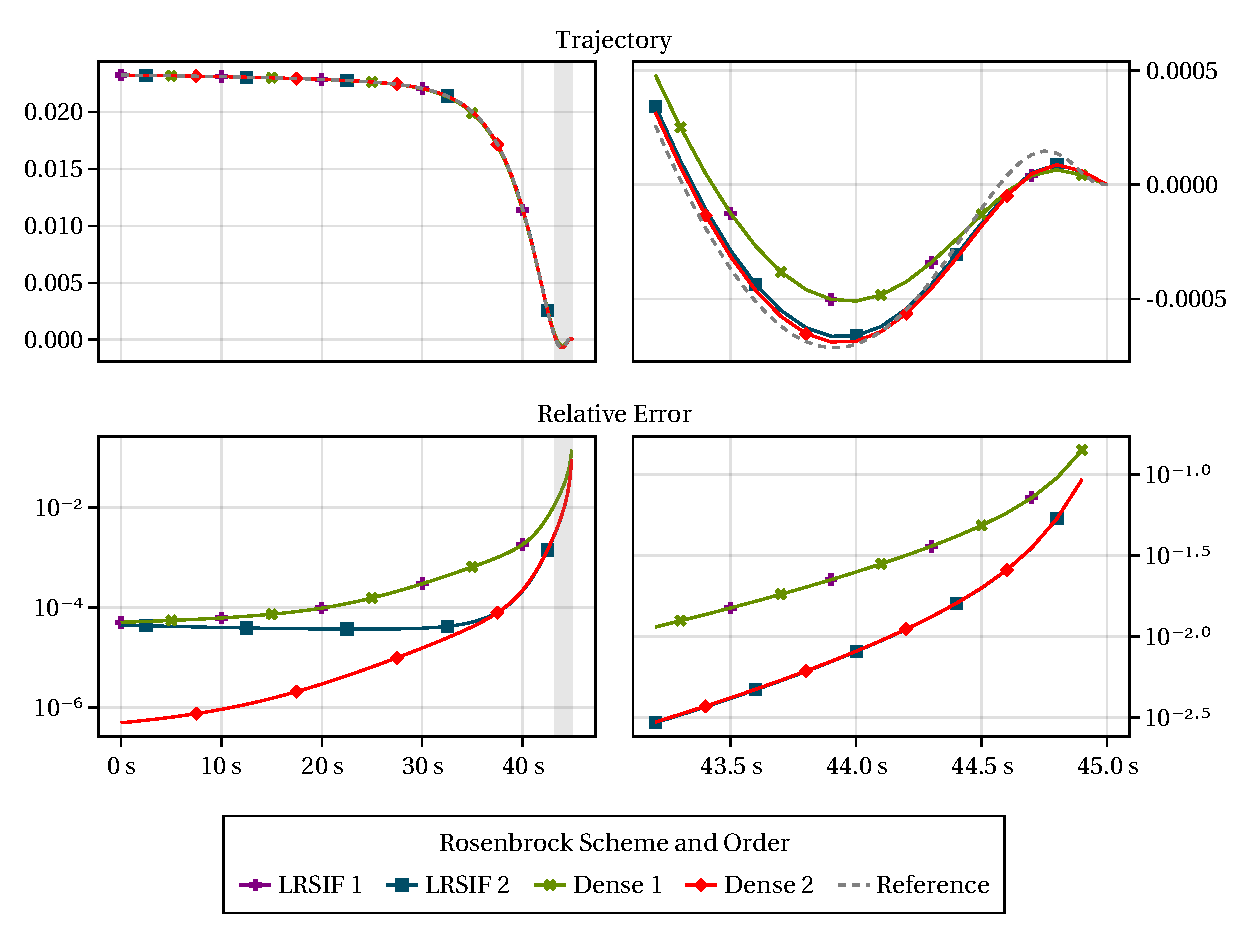
\includegraphics[width=\textwidth]{figures/fig_results_sequential.pdf}
  \caption[Rosenbrock method applied to Rail problem]{%
    Several Rosenbrock schemes applied to the problem of \autoref{thm:rail:parameters}.
    Each scheme performs 450 steps ($\tau = \SI{100}{\milli\second}$).
    Top: trajectory of $K_{1,77}$ (same as \cite[Fig.~1]{Lang2015}),
    % same as Lang2015, Fig. 1
    % Lang2017, Fig 6.1 used K_{1,71} instead
    bottom: relative error \eqref{eq:results:err:ref} compared to reference solution
    (900 steps of dense Rosenbrock scheme of order 4).
    Left: global time span $[\SI{0}{\second}, \SI{45}{\second}]$,
    right: zoom to $[\SI[round-mode=off]{43.2}{\second}, \SI{45}{\second}]$ (highlighted on the left).
  }
  \label{fig:results:sequential:rail}
\end{figure}

The problem of \ac{LRSIF}~2 can be confirmed with the (global) relative error
\begin{equation}
\label{eq:results:err:lr_v_dense}
  \frac{\norm{K_\text{\ac{LRSIF}}(t) - K_\text{Dense}(t)}_F}{\norm{K_\text{Dense}(t)}_F}
\end{equation}
between low-rank and dense variants of the same algorithm,
\cf~\autoref{fig:results:sequential:err}.
For \Ros{1} this value is within margin,
since $n \umach \approx 10^{-13}$.
However, for \Ros{2} there is a significant error from the very first iteration at $t=\SI[round-precision=1]{44.9}{\second}$.
This error stays about constant for the remainder of the time span.

\begin{figure}[tp]
  \centering
  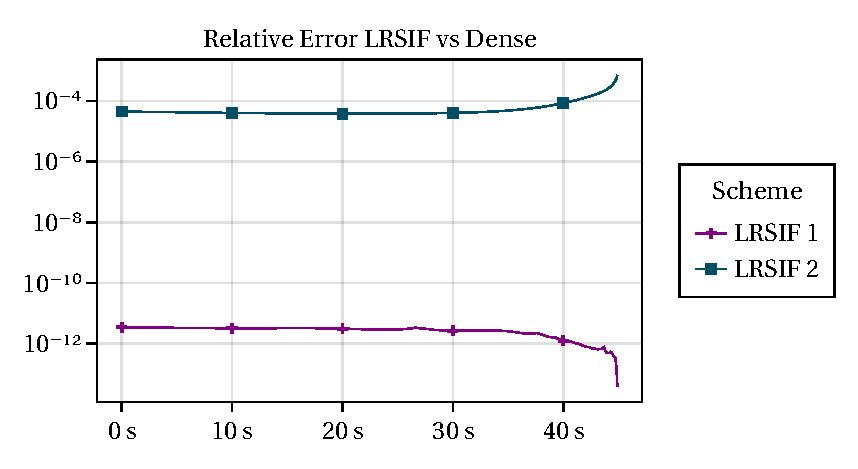
\includegraphics[width=0.75\textwidth]{figures/fig_results_sequential_err.pdf}
  \caption[Relative error between low-rank and dense solvers]{%
    Relative error \eqref{eq:results:err:lr_v_dense} in $K$ between low-rank and dense solvers
  }
  \label{fig:results:sequential:err}
\end{figure}

As mentioned in \autoref{thm:lowrank:rail},
the rank of $X$ should not get much larger than 113 along its trajectory.
\ac{LRSIF}~1 fulfills that expectation, as shown in \autoref{fig:results:sequential:rank}.
It grows quickly for $t > \SI{44}{\second}$ and seems to trend towards a plateau for $t< \SI{30}{\second}$.
\ac{LRSIF}~2, however, does not seem to stabilize,
which results in significantly larger ranks for about $t < \SI{40}{\second}$.

\begin{remark}
  \citeauthor{Lang2015}~\cite[63]{Lang2015} noted a problem with the low-rank version of \Ros{2} as well.
  The error behavior here looks similar to \cite[Fig~1]{Lang2015},
  keeping in mind that here the step size is $100\times$ larger
  and that the results are compared to dense solvers instead of \ac{LRCF} ones.
\end{remark}

\begin{figure}[tp]
  \centering
  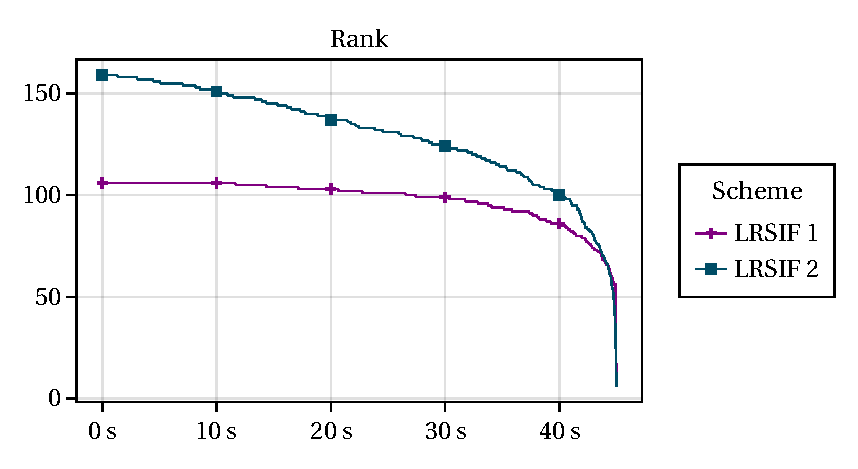
\includegraphics[width=0.7\textwidth]{figures/fig_results_sequential_rank.pdf}
  \caption[Numerical rank of low-rank sequential solutions to Rail problem]{%
    Numerical rank of low-rank sequential solutions $X$ to Rail problem,
    \cf~\cite[Figure~6.6b]{Lang2017}.
  }
  \label{fig:results:sequential:rank}
\end{figure}

The rank of the solution $X(t_n)$ has a major effect on the runtime of the next Rosenbrock step.
Recall that \Ros{1} leads to an \ac{ALE} whose right-hand is (a compression of) a \ac{LRSIF} of rank $q+r$
where $r := \rank X(t_n)$ denotes the rank of the previous Rosenbrock iterate.
Similarly, the right-hand side of the first stage of \Ros{2} is (a compression) of rank $q + 2r$.
The rank of the \ac{ADI} iterate thus grows by about that amount.
In the worst case, this causes a compression to be performed after every iteration of the \ac{ADI}.

\pagebreak

\subsection{Parareal Solvers}
\label{sec:results:parareal}

\autoref{fig:results:parareal:rail} shows the results of the parareal method described in \autoref{sec:pr}
for dense and \ac{LRSIF} algorithms and several order combinations.
Again, the schemes should perform identically for dense and \ac{LRSIF} storage.
As expected due to the problem discovered for \ac{LRSIF}~2,
this is true only for the parareal schemes of order 1/1 for their coarse/fine solver.
The reference solution has been computed with a dense order 4/4 parareal scheme.
Its $K_{1,77}$ trajectory is not shown as it would be indistinguishable from the other solutions.

\begin{figure}[tp]
  \centering
  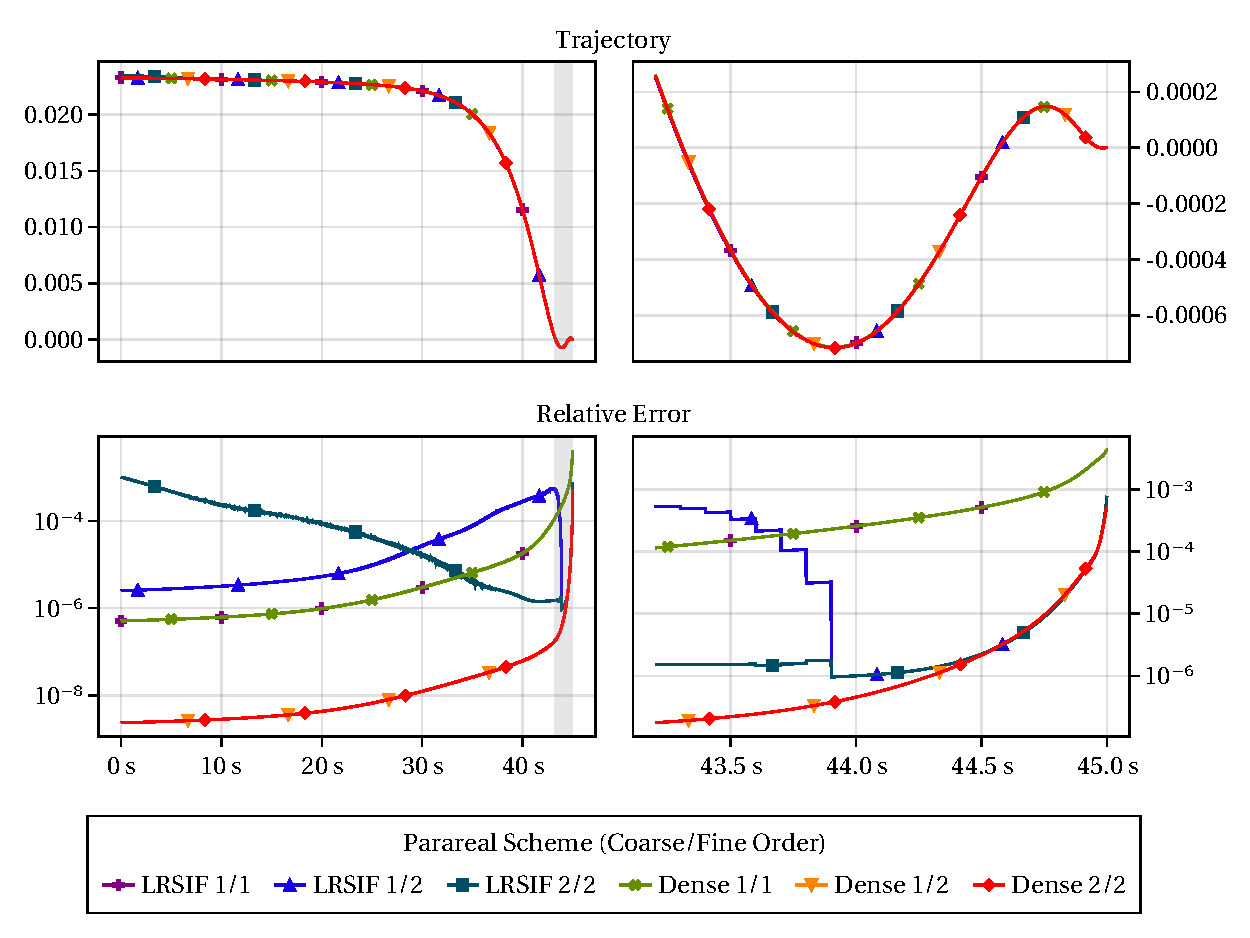
\includegraphics[width=\textwidth]{figures/fig_results_parareal.pdf}
  \caption[Parareal method applied to Rail problem]{%
    Several parareal schemes (Rosenbrock methods of given coarse/fine order)
    applied to the problem of \autoref{thm:rail:parameters},
    running on $N=450$ cores and
    computing up to $K=10$ refinements.
    Each scheme performs
    one coarse step ($\tau=\SI{100}{\milli\second}$) and
    100 fine steps ($\tau=\SI{1}{\milli\second}$) per stage.
    Top: trajectory of $K_{1,77}$ (same as \cite[Fig.~1]{Lang2015}),
    % same as Lang2015, Fig. 1
    % Lang2017, Fig 6.1 used K_{1,71} instead
    bottom: relative error \eqref{eq:results:err:ref} compared to reference solution
    (dense parareal scheme of order 4/4).
    Left: global time span $[\SI{0}{\second}, \SI{45}{\second}]$,
    right: zoom to $[\SI[round-mode=off]{43.2}{\second}, \SI{45}{\second}]$ (highlighted on the left).
  }
  \label{fig:results:parareal:rail}
\end{figure}

For the methods involving \ac{LRSIF}~2,
the relative error~\eqref{eq:results:err:ref} reveals
the typical discontinuities at the interval bounds
before convergence is reached,
\cf~\autoref{fig:pr:linear},
for $n > K = 10$ or $t \leq \SI[round-precision=1]{43.9}{\second}$.
But even for $t > \SI[round-precision=1]{43.9}{\second}$ the error of the low-rank variants is noticeably larger.
This effect has only been visible for $t < \SI{35}{\second}$ in the purely sequential setting,
\cf~\autoref{fig:results:sequential:rail}.
What looked like a more or less constant error in the previous subsection,
seems to be diverging in \autoref{fig:results:parareal:rail} for \ac{LRSIF}~2/2 as $t$ approaches $-\infty$,
which is in stark contrast to the otherwise downwards trend of the errors.
For about $t < \SI{28}{\second}$ the \ac{LRSIF}~2/2 solution is worse than the mixed order solution of \ac{LRSIF}~1/2.
Looking closely, the large error of \ac{LRSIF}~2/2 starts to become visible for $K_{1,77}$ around $t=\SI{0}{\second}$.


The rank of the solutions $X$ largely depends on the methods used,
\cf~\autoref{fig:results:parareal:rank}.
The parareal scheme \ac{LRSIF}~1/1 yields about the same ranks as the sequential \ac{LRSIF}~1.
Interestingly, the ranks of \ac{LRSIF}~1/2 are not much larger,
while showing the same plateau-effect.
This causes the runtimes $t_F(n, k_n)$ and $t_G(n, k_n)$ to not deviate too much for different $n$.
As can be seen in \autoref{fig:results:parareal:timeline},
all methods of order~1/1 and~1/2
reasonably fulfill the assumptions of the timeline model~\eqref{eq:impl:tpar} stated in \autoref{sec:impl:pr:warmup},
such that their timelines are close to the schematic in \autoref{fig:timeline:revised}.
This can be confirmed by the small error in $\hattpar$ in \autoref{tab:results:warmup}.
While for the dense methods this is to be expected,
it allows some observations to be made for the low-rank methods:
\begin{enumerate}
  \item
    \Ros{1} is barely affected by the larger rank,
    which causes \ac{LRSIF}~1/1 and \ac{LRSIF}~1/2 to have about the same ramp-up delay.
    This delay, however, is about \SI[round-precision=1]{0.2}{\second} larger than the overhead for the dense algorithms.
  \item
    Due to its two stages, \Ros{2} is more affected by the growing rank.
    Therefore, for \ac{LRSIF}~1/2 the runtime $t_F(n, k)$ is monotonic in $n$.
    Yet it is nearly constant in $k$,
    which causes the timeline diagram of \ac{LRSIF}~2/2
    to be narrow for early stages $n \leq 100$,
    and wider for later stages $n \geq 300$,
    without a noticeable gap between the refinements $k$.
\end{enumerate}
The second effect is visible for \ac{LRSIF}~1/1 as well, but not to that extent.

The rank of the solution $X$ obtained from the parareal scheme \ac{LRSIF}~2/2, however,
is even larger rank than the rank produced by the sequential \ac{LRSIF}~2,
while showing the same growth behavior (for decreasing $t$).
Neither of the methods of order 2/2 has a timeline diagram explained by~\eqref{eq:impl:tpar} or \autoref{fig:timeline:generic},
which is for the following reasons:
\begin{enumerate}[resume]
  \item
    Dense~2/2 does not fulfill the assumption that all stages $n$ compute the same number of refinements,
    \ie $k_n$ is not constant.
    Due to early convergence, \cf~\autoref{sec:impl:pr:conv},
    the last stage $n=N$ for example computes fewer refinements, $k_N = 7 < 10 = K$.
    This causes the runtime model~\eqref{eq:impl:tpar} to over-estimate the actual runtime,
    $\hattpar > \tpar$,
    as seen by the large error in \autoref{tab:results:warmup}.
  \item
    For \ac{LRSIF}~2/2 both runtimes $t_G(n, k)$ and $t_F(n, k)$ are monotonic in both $n$ (due to the growing rank) and $k$,
    while also having a big deviation from their median.
    The monotonicity in $k$ causes its timeline diagram to fan out,
    while the monotonicity in $n$ causes each \enquote{feathers} $k$ of the timeline diagram to be bent backwards.
    The resulting gaps between successive refinements $k$ on the final stage $n=N$ are not considered
    by the schematic timeline, \cf~\autoref{fig:timeline:revised}.
    Furthermore, the median over all $t_G(\optional{},\optional{})$ is much larger than,
    and therefore not a representative for $t_G(\optional{}, 0)$,
    which determines the slope of the $k=0$ face of the timeline.
    This causes the estimated ramp-up delay $\trampup$ to become negative.
    Both effects, the gaps on stage $n=N$ as well as $\trampup<0$,
    attribute to the runtime model~\eqref{eq:impl:tpar} under-estimating the actual runtime,
    $\hattpar < \tpar$,
    as seen by the large error in \autoref{tab:results:warmup}.
\end{enumerate}
The timeline diagram of the Dense~4/4 reference solution is shown in \autoref{fig:impl:restart},
which does not fulfill all the assumptions due to early convergence.

\begin{figure}[tp]
  \centering
  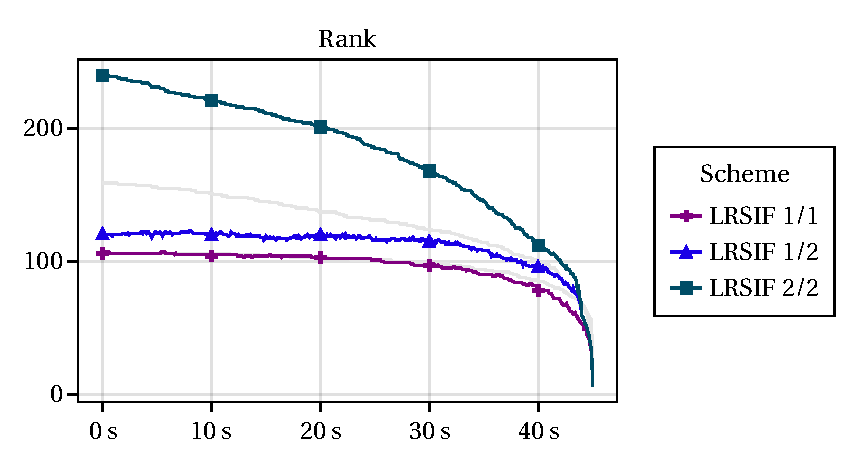
\includegraphics[width=0.7\textwidth]{figures/fig_results_parareal_rank.pdf}
  \caption[Numerical rank of low-rank parareal solutions to Rail problem]{%
    Numerical rank of low-rank parareal solutions to Rail problem,
    \cf~\cite[Figure~6.6b]{Lang2017}.
    Only values at parareal interfaces $t_n$ are shown,
    which coincide with the time steps of the sequential solutions.
    The numerical ranks of \autoref{fig:results:sequential:rail} are shown in the background.
  }
  \label{fig:results:parareal:rank}
\end{figure}

\begin{figure}[tp]
  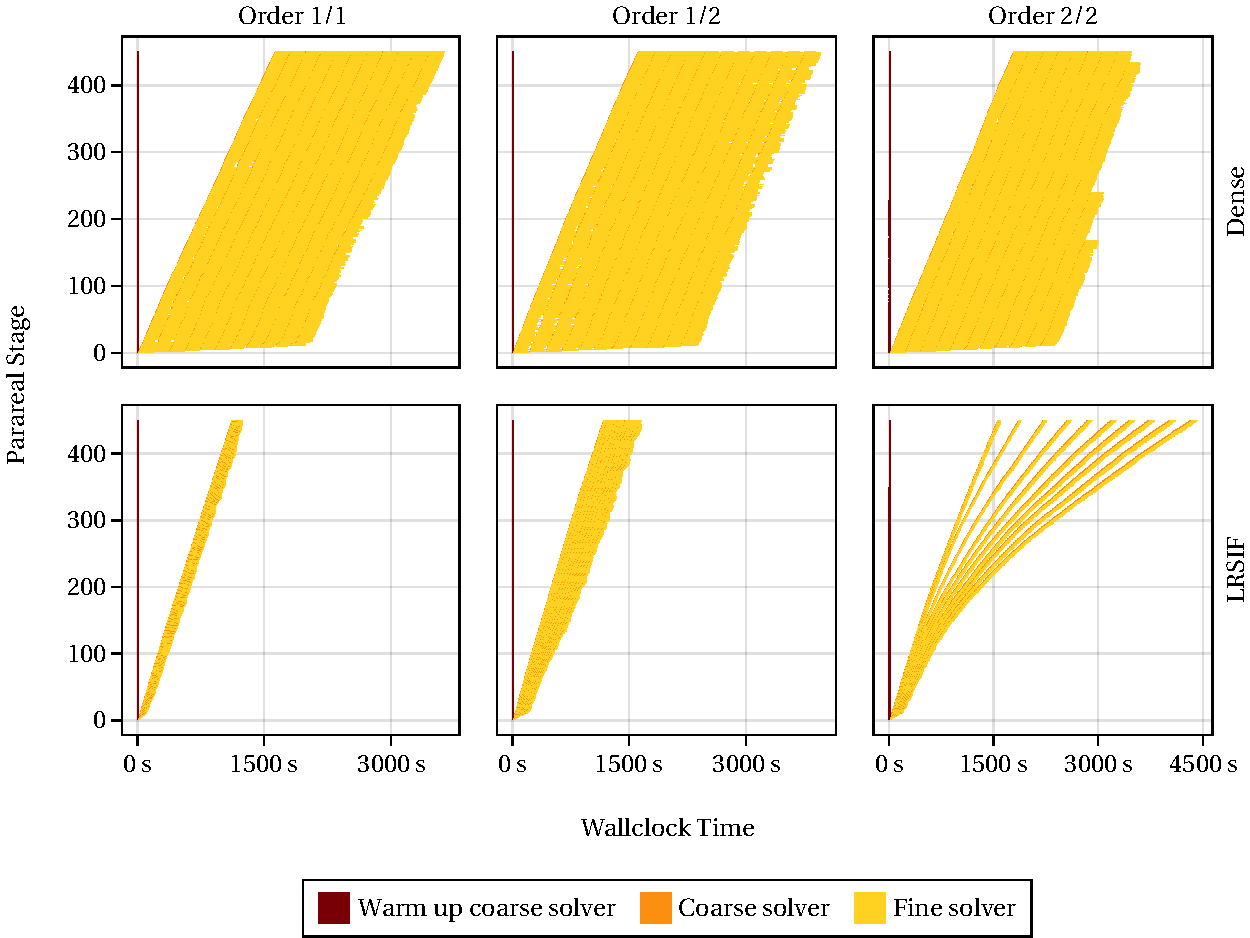
\includegraphics[width=\textwidth]{figures/fig_timeline_all.pdf}
  \caption[Timeline diagrams for parareal method applied to Rail problem]{%
    Timeline diagrams for the parareal methods applied to Rail problem.
    The schemes of coarse/fine order are as described in \autoref{fig:results:parareal:rail}.
  }
  \label{fig:results:parareal:timeline}
\end{figure}

\begin{table}[p]
  \centering
  \begin{tabular}{%
    l
    S[table-format=2] % k
    S[table-format=2.2] % warm-up
    S[table-format=-1.2] % ramp-up
    S[table-format=1.2] % G
    S[table-format=3.2] % F
    S[table-format=4.2] % par
    S[table-format=4.2] % par est
    S[round-precision=3, round-minimum=0.001, table-format=<1.3, scientific-notation=fixed, fixed-exponent=0] % err
  }
    \toprule
    Solver &
    {$k_N$} &
    {$\twarmup$} &
    {$\trampup$} &
    {$t_G$} &
    {$t_F$} &
    {$\tpar$} &
    {$\hattpar$} &
    {$\abs*{\frac{\hattpar-\tpar}{\tpar}}$} \\
    \midrule
    %TODO: Add uncertainties for low-rank t_F and t_G?
    LRSIF 1/1 & 10 & 18.126309871673584 & 1.9820044045989924 & 0.47998499870300293 & 9.849883079528809 & 1243.838875055313 & 1239.1701052194185 & 0.003753516576403047 \\
LRSIF 1/2 & 10 & 18.344510078430176 & 2.043351598200129 & 0.5375161170959473 & 32.58289909362793 & 1659.4842681884766 & 1543.5220331625312 & 0.06987847806025413 \\
LRSIF 2/2 & 10 & 21.727890968322754 & -1.6257711417956449 & 5.062106132507324 & 30.97498106956482 & 4417.833864927292 & 1959.4244898788647 & 0.5564739304855881 \\

    \addlinespace
    Dense 1/1 & 10 & 19.763540983200073 & 1.7398977895621996 & 1.8599169254302979 & 178.98965120315552 & 3627.2994508743286 & 3627.1654952188373 & 3.6929858509193245e-5 \\
Dense 1/2 & 10 & 19.545176029205322 & 1.7246065049500667 & 1.8416509628295898 & 209.07670402526855 & 3956.8617849349976 & 3942.621290436301 & 0.00359893654939238 \\
Dense 2/2 & 7 & 28.62309694290161 & 1.7665315399191162 & 2.167254090309143 & 209.65867733955383 & 3602.3622279167175 & 4126.744622183802 & 0.14556625932932343 \\

    \addlinespace
    Dense 4/4 & 4 & 28.806522130966187 & 1.6859412150818418 & 2.753262996673584 & 268.64974904060364 & 3381.8760890960693 & 5009.128286834284 & 0.48116848603201123 \\

    \bottomrule
  \end{tabular}
  \caption[Timeline measurements for parareal algorithm, $N=450$, $K=10$]{%
    Timeline measurements for parareal algorithm, $N=450$, $K=10$.
    All measurements and estimates are as in \autoref{tab:impl:warmup}.
    The first column denotes the parareal scheme (coarse/fine order).
    Refer to Figures \ref{fig:results:parareal:timeline} and \ref{fig:impl:restart} for the corresponding timelines.
  }
  \label{tab:results:warmup}
\end{table}

\begin{table}[p]
  \centering
  \begin{tabular}{%
    l
    S[table-format=4.2] % par
    S[table-format=6.2] % seq est
    S[table-format=2.2] % speedup
    S[round-precision=3, round-minimum=0.001, table-format=1.3, scientific-notation=fixed, fixed-exponent=0] % efficiency
  }
    \toprule
    Solver &
    {$\tpar$} &
    {$\hattseq$} &
    {$\frac{\hattseq}{\tpar}$} &
    {$\frac{\hattseq}{N\cdot\tpar}$} \\
    \midrule
    LRSIF 1/1 & 1243.838875055313 & 4313.1015791893005 & 3.4675725816959195 & 0.007705716848213155 \\
LRSIF 1/2 & 1659.4842681884766 & 14054.911208629608 & 8.469445283727943 & 0.018820989519395426 \\
LRSIF 2/2 & 4417.833864927292 & 24565.040289878845 & 5.560426453538251 & 0.012356503230085001 \\

    \addlinespace
    Dense 1/1 & 3627.2994508743286 & 75037.70862150192 & 20.686935180776086 & 0.0459709670683913 \\
Dense 1/2 & 3956.8617849349976 & 84595.60539913177 & 21.379469386879656 & 0.04750993197084368 \\
Dense 2/2 & 3602.3622279167175 & 89274.93912768364 & 24.78233266933632 & 0.05507185037630293 \\

    \addlinespace
    Dense 4/4 & 3381.8760890960693 & 115091.05863285065 & 34.03171955469633 & 0.07562604345488073 \\

    \bottomrule
  \end{tabular}
  \caption[Speed-up and parallel efficiency of parareal algorithm, $N=450$, $K=10$]{%
    Speed-up and parallel efficiency of parareal algorithm, $N=450$, $K=10$.
    This table complements \autoref{tab:results:warmup}.
    The sequential runtime $\hattseq$ is estimated according to~\eqref{eq:impl:tseq}.
    The parallel efficiency is evaluated for $N$ processors.
  }
  \label{tab:impl:pr:speedup}
\end{table}

\subsection{Runtime and Storage Size}

Refer to \autoref{tab:results:runtime} for the runtime and storage size of all resulting data sets.
Note that the ratios of the sizes of the data sets resulting from
sequential order~1 and parareal order~1/1
fit well to the estimated~1/3 of \autoref{thm:lowrank:rail}.
The other ratios are skewed by the rank problem of \ac{LRSIF}~\Ros{2}.

\begin{table}
  \centering
  \begin{tabular}{%
    lc
    % tau
    S[table-format=3]
    % runtime
    S[table-format=4]
    S[table-format=4]
    % size
    S[table-format=2.3, round-precision=3]
    S[table-format=2.3, round-precision=3]
  }
    \toprule
    &&&
    \multicolumn{2}{c}{Runtime [\si{\second}]} &
    \multicolumn{2}{c}{Size [\si{\gibi\byte}]} \\
    \cmidrule(rl){4-5}
    \cmidrule(rl){6-7}
    Solver & Order & {Resolution [\si{\milli\second}]} &
    {Dense} & {LRSIF} &
    {Dense} & {LRSIF} \\
    \midrule % jobid dense, lowrank
    Sequential & 1 & 100 & 217 & 599 & 0.472 & 0.165 \\ % 351941, 351939
    Sequential & 2 & 100 & 602 & 708 & 0.472 & 0.231 \\ % 351942, 351940
    \addlinespace
    Parareal & 1/1 & 1 & 4724 & 2366 & 47.047 & 15.971 \\ % 351236, 351158
    Parareal & 1/2 & 1 & 5057 & 2775 & 47.047 & 19.084 \\ % 351235, 351167
    Parareal & 2/2 & 1 & 4730 & 5519 & 47.047 & 35.161 \\ % 351290, 351160
    \addlinespace
    Sequential & 4 & 50 & 1785 & {--} & 0.942 & {--} \\ % 351965
    Parareal & 4/4 & 1 & 4512 & {--} & 47.047 & {--} \\ % 351270
    \bottomrule
  \end{tabular}
  \caption[Runtime and storage requirements]{%
    Overall runtime (as reported by Slurm)
    including time to write results to disk,
    and storage requirements of solutions to Rail benchmark~\cite{morwiki_steel}.
    The resolution is the step size $\tau$ of the (fine) solver.
    The storage size includes both $X$ and $K$ trajectories,
    storing only $K$ would result in substantially smaller files.
  }
  \label{tab:results:runtime}
\end{table}


\chapter{Conclusion}
\label{sec:conclusion}

\sisetup{round-precision=1}

This thesis has given a brief overview on the \ac{DRE} arising in optimal control in \autoref{sec:HJT},
and how to handle large-scale problems in general in \autoref{sec:matrixeq}.
Then, \autoref{sec:ros} has shown that
applying the classical Rosenbrock method to the matrix-valued \ac{DRE}
results in the stage equations being \acp{ALE}
having absolute terms in \ac{LRSIF}.
When solving these equations with the \ac{ADI} method,
the solution's low-rank structure causes the \ac{ADI} sub-steps to operate on different low-rank factors.
Due to the symmetry of the solution,
and the particular choice of \ac{ADI} parameters,
these low-rank factors remain identical for every \ac{ADI} iteration.
Therefore, effectively only one of two \ac{ADI} sub-steps has to be performed every iteration.
It was further shown how the general structure of the \ac{ADI} allows to efficiently iterate the low-rank residual alongside the solution,
how to evaluate its norm without assembling the full residual matrix,
and how to handle complex parameters using real arithmetic for the iterates.
Lastly, \autoref{sec:ADI} described how to choose \ac{ADI} parameters based on quantities computed during the \ac{ADI},
\ie independent from user input.

\autoref{sec:pr} and parts of \autoref{sec:impl} addressed the parareal method.
It was shown how to apply the method to \acp{LRSIF}.
When using the parareal method from a \ac{JIT} compiled language like Julia,
it is crucial that the coarse solver is already compiled before the parareal iteration starts.
Otherwise, the overhead of compilation scales with the number of parareal stages~$N$,
rendering the method infeasible for practical use.
Still, there is another linear overhead of about $\trampup \approx \SI{1.8}{\second}$ per stage,
caused by the compilation of communication code.
Overall, the efficiency is very low:
less than \SI{2}{\percent} for the low-rank algorithms and
\SIrange{4.6}{7.6}{\percent} for the dense algorithms.
Yet, the speed-up is very noticeable:
\eg more than \num{34} for the most expensive dense algorithm,
\cf~\autoref{tab:impl:pr:speedup}.
These metrics would be larger for finer temporal resolutions,
a lower ramp-up delay~$\trampup$,
or more advanced scheduling strategies.
The latter would especially benefit the low-rank algorithms.

Numerically, the \ac{LRSIF} version of \Ros{1} performed just like its dense counterpart.
The problems with the \ac{LRSIF} version of \Ros{2} as noted by \citeauthor*{Lang2015}~\cite{Lang2015,Lang2017} have been reproduced in Julia.
They are especially severe in a parareal context,
which makes the comparison of runtime and derived metrics involving this method basically pointless.
However, investigation is difficult as the level of introspection
currently possible using \code{DifferentialRicccatiEquations.jl} is quite poor:
it does not track the actual rank of the \ac{ALE} right-hand sides,
nor the number of \ac{ADI} iterations or number of \ac{LRSIF} compressions performed.
Furthermore, the thresholds when to perform a \ac{LRSIF} compression are not configurable yet,
would be necessary to apply the algorithms to large-scale problems.

Julia allows for user-friendly abstractions while still providing good performance.
In particular, dynamic dispatch and extendable standard operators like \julia{(+)} are very useful.
It was mostly fun to work with, but could be improved in the following aspects.
%The tooling around the language isn't as mature.
First, the runtime is too forgiving when errors occur,
especially in a distributed environment.
There is no simple way to make it more strict, \eg to crash all worker processes on a single unhandled error.
Second, the thread-safety of the standard library could be improved.
This would allow \code{ParaReal.jl} to perform communication asynchronously.
Third, Julia determines a suitable text representation of an object (\eg \julia{display()}) based on the number of terminal rows available.
This applies to errors as well, causing \eg grouped errors due to a pipeline failure to only print the first error,
which may not be the root cause of the problem.
Subsequent errors are lost in an ellipsis (\enquote{\ldots{} and 41 more exceptions}).
In a truly headless setting,
\eg inside a job executed by a job scheduling system like Slurm,\footnote{\url{https://slurm.schedmd.com/overview.html}}
all errors should be printed by default (or \enquote{\ldots{} and 41 identical exceptions more}).
Having these issues in mind,
and considering that Julia is still a very young language compared to the ones dominant in high-performance computing,
Julia is an option worth considering for future projects in science and engineering.


% -----------------------------------------------------------------------------
\appendix
%\chapter{Notes}

\begin{align}
  E\dot{X} &= AX + BU \\
  Y &= CX + DU \\
  X(t_0) &= X_0
\end{align}

\section{Equation Types}
\subsection{Standard}

Differential and algebraic Riccati equations:
\begin{align}
  \dot{X} &= A^\T X + XA - XSX + W \\
  0 &= A^\T X + XA - XSX + W \\
\intertext{Differential and algebraic Lyapunov equations:}
  \dot{X} &= A^\T X + XA + W \\
  0 &= A^\T X + XA + W
\end{align}

\subsection{Generalized}

Substituting $X\gets E^\T XE$ leads to generalized equations.
Generalized differential and algebraic Riccati equations (assuming $\dot E = 0$):
\begin{align}
  E^\T \dot{X}E &= A^\T XE + E^\T XA - E^\T XSXE + W \\
  0 &= A^\T XE + E^\T XA - E^\T XSXE + W \\
\intertext{Generalized differential and algebraic Lyapunov equations:}
  E^\T \dot{X}E &= A^\T XE + E^\T XA + W \\
  0 &= A^\T XE + E^\T XA + W \\
\end{align}

\cite{Lang2018}

\section{Alternating Directions Method}

\section{Software}

\cite{DrWatson}

\section{Hamilton-Jacobi Theory}

Consider the optimal control problem
\begin{equation}
  \everymath{\displaystyle}
  \begin{array}{cl}
    \min_u & \int_{t_0}^{t_f} \ell(t, x(t), u(t)) \dt + m(t_f, x(t_f)) \\
    \text{s.t.} & \dot{x} = f(t,x,u), \enspace x(t_0) = x_0
  \end{array}
  \label{eq:optimal-control}
\end{equation}
using \emph{state}~$x:\R\to\R^n$, system \emph{control}~$u:\R\to\R^m$,
and scalar cost functions~$\ell$ and $m$.
An optimal control $u^*$ solving \eqref{eq:optimal-control} may be defined by means of the
\emph{value function}~$V:\R\times\R^n\to\R$ satisfying the \emph{Hamilton-Jacobi} equation
\begin{equation}
  V_t(t,x) + H(t,x,u^h,V_x^\T(t,x)) = 0.
  \label{eq:hamilton-jacobi}
\end{equation}
The \emph{Hamiltonian} $H:\R\times\R^n\times\R^m\times\R^n\to\R$ is given by
\begin{equation}
  H(t,x,u,\lambda) = \ell(t,x,u) + \lambda^\T f(t,x,u)
\end{equation}
and $u^h = u^h(t,x,V_x^\T)$ denotes the $H$-minimizing control.
In the context of the linear dynamical system
\begin{equation}
  \begin{aligned}
    E\dot{x} &= Ax + Bu \\
    y &= Cx
  \end{aligned}
\end{equation}
together with the state transformation $z=Ex$ and particular choices for $\ell$ and $m$,
making the ansatz
\begin{equation}
  V(t,z) = z^\T Xz + w^\T z + v
\end{equation}
and solving for $X:\R\to\R^{n,n}$, $w:\R\to\R^n$, $v:\R\to\R$ will eventually
yield a \emph{generalized differential Riccati equation} in $X$ as well as
ordinary differential equations in $w$ and $v$.

\chapter{ADI Reordering Following \citeauthor{Li2002}}
\label{sec:li2002}

\citeauthor{Li2002} \cite{Li2002} propose a reordering of the terms to simplify computations.
The exact motivation will become apparent when applying the \ac{ADI} method to an \ac{ALE}.
For an initial value of $x^0 = 0$,
the \ac{ADI} reads:
\begin{align*}
  x^{k+1}
  &= G_k x^k + B_k b \\
  &= G_k G_{k-1} x^{k-1} + (G_k B_{k-1} + B_k) b \\
  &= G_k G_{k-1} (G_{k-2} x^{k-2} + B_{k-2}b) + (G_k B_{k-1} + B_k) b \\
  &= G_k \cdots G_{k-2} x^{k-2} + (G_k G_{k-1} B_{k-2} + G_k B_{k-1} + B_k) b \\
  &\vdotswithin{=} \\
  &= \underbrace{G_k \cdots G_0 x^0}_0 {} + (G_k \cdots G_1 B_0 + \ldots + G_k B_{k-1} + B_k) b \\
\intertext{%
  \autoref{thm:adi:permutation} allows to introduce a permutation $\sigma$ of $\Set{0,\ldots,k}$.
  Thus:
}
  &= (G_{\sigma(k)} \cdots G_{\sigma(1)} B_{\sigma(0)} + \ldots + G_{\sigma(k)} B_{\sigma(k-1)} + B_{\sigma(k)}) b \\
\intertext{%
  Choosing $\sigma = \sigma_k : i \mapsto k-i$,
  and exploiting that $G_* B_* = B_* G_*$ commute,
  yields:
}
  &= (G_0 \cdots G_{k-1} B_k + \ldots + G_0 B_1 + B_0) b \\
  &= (B_k G_{k-1} \cdots G_0 + \ldots + B_1 G_0 + B_0) b \\
\intertext{%
  Further utilizing $G_k := M_k^{-1} N_k = N_k M_k^{-1}$ and $B_k := M_k^{-1}$ leads to:
}
  &= \big( M_k^{-1} (N_{k-1} M_{k-1}^{-1}) \cdots (N_0 M_0^{-1}) + \ldots + M_1^{-1} (N_0 M_0^{-1}) + M_0^{-1} \big) b \\
  &= \big( (M_k^{-1} N_{k-1}) \cdots (M_1^{-1} N_0) M_0^{-1} + \ldots + (M_1^{-1} N_0) M_0^{-1} + M_0^{-1} \big) b \\
  &= \underbrace{
    (M_k^{-1} N_{k-1}) \cdots (M_1^{-1} N_0) M_0^{-1} b
  }_{v^k}
  + \underbrace{
    \big( \ldots + (M_1^{-1} N_0) M_0^{-1} + M_0^{-1} \big) b
  }_{x^k}
\end{align*}
Regrouping reveals:
\begin{equation*}
\left\{
\begin{aligned}
  x^{k+1} &= x^k + v^k &
  x^0 &= 0 \\
  v^k &= (M_k^{-1} N_{k-1}) v^{k-1} &
  v^0 &= M_0^{-1} b
\end{aligned}
\right.
\end{equation*}


%\chapter{Control Theory}

\begin{itemize}
  \item
    exponentially stable matrix,
  \item
    stabilizable matrix pair,
  \item
    reachable/controllable/unobservable state,
  \item
    detectable/reachable/observable system,
    \etc
\end{itemize}

\chapter{Kronecker Product and Vectorization}
\label{sec:vectorization}

This chapter gives some more details on how to apply the concept's presented in \autoref{sec:adi:1step} to \acp{ALE},
in particular how right-multiplication $X \mapsto XA^\HT$ can be described as a left-multiplication.
The key ingredients for this are \emph{vectorization} $\vec : \R^{m\times n} \to \R^{mn}$,
\eg for $X=(x_1,\ldots, x_n)$ with $x_i\in\R^m$
\begin{equation}
  \vec(X) := \begin{bmatrix}
    x_1 \\
    \vdots \\
    x_n
  \end{bmatrix}
\end{equation}
and the \emph{Kronecker product} $\otimes : \R^{m\times n} \times \R^{p\times q} \to \R^{mp \times nq}$,
\begin{equation}
  A \otimes B := \begin{bmatrix}
    a_{11} B & \cdots & a_{1n} B \\
    \vdots   & \ddots & \vdots \\
    a_{m1} B & \cdots & a_{mn} B
  \end{bmatrix}
  .
\end{equation}
Then, without a proof, the following holds:

\begin{proposition}[Kronecker Product]
  Let $A, B, C$ be complex-valued matrices of compatible size. Then
  \begin{equation*}
    \vec(ABC) = (C^\T \otimes A) \vec(B)
    .
  \end{equation*}
\end{proposition}

In particular, in the context of \autoref{sec:adi:ale}
and the \ac{ALE}~\eqref{eq:adi:ale}, it is
\begin{gather}
  \Lyap_L \cong \vec(X) \mapsto \vec(AX) = (I \otimes A) \vec(X) \\
  \Lyap_R \cong \vec(X) \mapsto \vec(XA^\HT) = (\conj A \otimes I) \vec(X)
\end{gather}
such that the \ac{ALE}
\begin{equation}
  \Lyap(X) = \Lyap_L(X) + \Lyap_R(X) = -W
\end{equation}
is equivalent to
\begin{equation}
  (I \otimes A + \conj A \otimes I) \vec(X) = -\vec(W)
  .
\end{equation}


% -----------------------------------------------------------------------------
\backmatter
\printbibliography

\end{document}
